\documentclass{report}

%%%%%%%%%%%%%%%%%%%%%%%%%%%%%%%%%
% PACKAGE IMPORTS
%%%%%%%%%%%%%%%%%%%%%%%%%%%%%%%%%


\usepackage[tmargin=2cm,rmargin=1in,lmargin=1in,margin=0.85in,bmargin=2cm,footskip=.2in]{geometry}
\usepackage{amsmath,amsfonts,amsthm,amssymb,mathtools}
\usepackage[varbb]{newpxmath}
\usepackage{xfrac}
\usepackage[makeroom]{cancel}
\usepackage{mathtools}
\usepackage{bookmark}
\usepackage{enumitem}
\usepackage{listings}
\usepackage{hyperref,theoremref}
\hypersetup{
	pdftitle={Assignment},
	colorlinks=true, linkcolor=myp,
	bookmarksnumbered=true,
	bookmarksopen=true
}
\usepackage[most,many,breakable]{tcolorbox}
\usepackage{xcolor}
\usepackage{varwidth}
\usepackage{varwidth}
\usepackage{etoolbox}
%\usepackage{authblk}
\usepackage{nameref}
\usepackage{multicol,array}
\usepackage{tikz-cd}
\usepackage[ruled,vlined,linesnumbered]{algorithm2e}
\usepackage{comment} % enables the use of multi-line comments (\ifx \fi) 
\usepackage{import}
\usepackage{xifthen}
\usepackage{pdfpages}
\usepackage{transparent}
\usepackage{afterpage}
\usepackage{tikz}
\usetikzlibrary{er, fit}
\usetikzlibrary{positioning}

\newcommand\mycommfont[1]{\footnotesize\ttfamily\textcolor{myp}{#1}}
\SetCommentSty{mycommfont}
\newcommand{\incfig}[1]{%
    \def\svgwidth{\columnwidth}
    \import{./figures/}{#1.pdf_tex}
}

\usepackage{tikzsymbols}
\renewcommand\qedsymbol{$\Laughey$}


%\usepackage{import}
%\usepackage{xifthen}
%\usepackage{pdfpages}
%\usepackage{transparent}

%%%%%%%%%%%%%%%%%%%%%%%%%%%%%%
% BLANK PAGE
%%%%%%%%%%%%%%%%%%%%%%%%%%%%%%

\newcommand\blankpage{%
    \null
    \thispagestyle{empty}%
    \addtocounter{page}{-1}%
    \newpage
}

%%%%%%%%%%%%%%%%%%%%%%%%%%%%%%
% LISTING
%%%%%%%%%%%%%%%%%%%%%%%%%%%%%%

\lstdefinestyle{SQL}{
  language=SQL,
  basicstyle=\ttfamily,
  keywordstyle=\color{blue},
  commentstyle=\color{green},
  stringstyle=\color{red},
  numbers=left,
  numberstyle=\tiny\color{gray},
  stepnumber=1,
  numbersep=5pt,
  breaklines=true,
  showstringspaces=false,
  frame=single,
  captionpos=b
}

%%%%%%%%%%%%%%%%%%%%%%%%%%%%%%
% SELF MADE COLORS
%%%%%%%%%%%%%%%%%%%%%%%%%%%%%%

\definecolor{myg}{RGB}{56, 140, 70}
\definecolor{myb}{RGB}{45, 111, 177}
\definecolor{myr}{RGB}{199, 68, 64}
\definecolor{mytheorembg}{HTML}{F2F2F9}
\definecolor{mytheoremfr}{HTML}{00007B}
\definecolor{mylenmabg}{HTML}{FFFAF8}
\definecolor{mylenmafr}{HTML}{983b0f}
\definecolor{mypropbg}{HTML}{f2fbfc}
\definecolor{mypropfr}{HTML}{191971}
\definecolor{myexamplebg}{HTML}{F2FBF8}
\definecolor{myexamplefr}{HTML}{88D6D1}
\definecolor{myexampleti}{HTML}{2A7F7F}
\definecolor{mydefinitbg}{HTML}{E5E5FF}
\definecolor{mydefinitfr}{HTML}{3F3FA3}
\definecolor{notesred}{RGB}{0,162,0}
\definecolor{myp}{RGB}{197, 92, 212}
\definecolor{mygr}{HTML}{2C3338}
\definecolor{myred}{RGB}{127,0,0}
\definecolor{myyellow}{RGB}{169,121,69}
\definecolor{myexercisebg}{HTML}{F2FBF8}
\definecolor{myexercisefg}{HTML}{88D6D1}

%%%%%%%%%%%%%%%%%%%%%%%%%%%%
% TCOLORBOX SETUPS
%%%%%%%%%%%%%%%%%%%%%%%%%%%%

\setlength{\parindent}{1cm}
%================================
% THEOREM BOX
%================================

\tcbuselibrary{theorems,skins,hooks}
\newtcbtheorem[number within=section]{Theorem}{Teorema}
{%
	enhanced,
	breakable,
	colback = mytheorembg,
	frame hidden,
	boxrule = 0sp,
	borderline west = {2pt}{0pt}{mytheoremfr},
	sharp corners,
	detach title,
	before upper = \tcbtitle\par\smallskip,
	coltitle = mytheoremfr,
	fonttitle = \bfseries\sffamily,
	description font = \mdseries,
	separator sign none,
	segmentation style={solid, mytheoremfr},
}
{th}

\tcbuselibrary{theorems,skins,hooks}
\newtcbtheorem[number within=chapter]{theorem}{Theorem}
{%
	enhanced,
	breakable,
	colback = mytheorembg,
	frame hidden,
	boxrule = 0sp,
	borderline west = {2pt}{0pt}{mytheoremfr},
	sharp corners,
	detach title,
	before upper = \tcbtitle\par\smallskip,
	coltitle = mytheoremfr,
	fonttitle = \bfseries\sffamily,
	description font = \mdseries,
	separator sign none,
	segmentation style={solid, mytheoremfr},
}
{th}


\tcbuselibrary{theorems,skins,hooks}
\newtcolorbox{Theoremcon}
{%
	enhanced
	,breakable
	,colback = mytheorembg
	,frame hidden
	,boxrule = 0sp
	,borderline west = {2pt}{0pt}{mytheoremfr}
	,sharp corners
	,description font = \mdseries
	,separator sign none
}

%================================
% Corollery
%================================
\tcbuselibrary{theorems,skins,hooks}
\newtcbtheorem[number within=section]{Corollary}{Corollary}
{%
	enhanced
	,breakable
	,colback = myp!10
	,frame hidden
	,boxrule = 0sp
	,borderline west = {2pt}{0pt}{myp!85!black}
	,sharp corners
	,detach title
	,before upper = \tcbtitle\par\smallskip
	,coltitle = myp!85!black
	,fonttitle = \bfseries\sffamily
	,description font = \mdseries
	,separator sign none
	,segmentation style={solid, myp!85!black}
}
{th}
\tcbuselibrary{theorems,skins,hooks}
\newtcbtheorem[number within=chapter]{corollary}{Corollary}
{%
	enhanced
	,breakable
	,colback = myp!10
	,frame hidden
	,boxrule = 0sp
	,borderline west = {2pt}{0pt}{myp!85!black}
	,sharp corners
	,detach title
	,before upper = \tcbtitle\par\smallskip
	,coltitle = myp!85!black
	,fonttitle = \bfseries\sffamily
	,description font = \mdseries
	,separator sign none
	,segmentation style={solid, myp!85!black}
}
{th}


%================================
% LENMA
%================================

\tcbuselibrary{theorems,skins,hooks}
\newtcbtheorem[number within=section]{Lenma}{Lenma}
{%
	enhanced,
	breakable,
	colback = mylenmabg,
	frame hidden,
	boxrule = 0sp,
	borderline west = {2pt}{0pt}{mylenmafr},
	sharp corners,
	detach title,
	before upper = \tcbtitle\par\smallskip,
	coltitle = mylenmafr,
	fonttitle = \bfseries\sffamily,
	description font = \mdseries,
	separator sign none,
	segmentation style={solid, mylenmafr},
}
{th}

\tcbuselibrary{theorems,skins,hooks}
\newtcbtheorem[number within=chapter]{lenma}{Lenma}
{%
	enhanced,
	breakable,
	colback = mylenmabg,
	frame hidden,
	boxrule = 0sp,
	borderline west = {2pt}{0pt}{mylenmafr},
	sharp corners,
	detach title,
	before upper = \tcbtitle\par\smallskip,
	coltitle = mylenmafr,
	fonttitle = \bfseries\sffamily,
	description font = \mdseries,
	separator sign none,
	segmentation style={solid, mylenmafr},
}
{th}


%================================
% PROPOSITION
%================================

\tcbuselibrary{theorems,skins,hooks}
\newtcbtheorem[number within=section]{Prop}{Proposition}
{%
	enhanced,
	breakable,
	colback = mypropbg,
	frame hidden,
	boxrule = 0sp,
	borderline west = {2pt}{0pt}{mypropfr},
	sharp corners,
	detach title,
	before upper = \tcbtitle\par\smallskip,
	coltitle = mypropfr,
	fonttitle = \bfseries\sffamily,
	description font = \mdseries,
	separator sign none,
	segmentation style={solid, mypropfr},
}
{th}

\tcbuselibrary{theorems,skins,hooks}
\newtcbtheorem[number within=chapter]{prop}{Proposition}
{%
	enhanced,
	breakable,
	colback = mypropbg,
	frame hidden,
	boxrule = 0sp,
	borderline west = {2pt}{0pt}{mypropfr},
	sharp corners,
	detach title,
	before upper = \tcbtitle\par\smallskip,
	coltitle = mypropfr,
	fonttitle = \bfseries\sffamily,
	description font = \mdseries,
	separator sign none,
	segmentation style={solid, mypropfr},
}
{th}


%================================
% CLAIM
%================================

\tcbuselibrary{theorems,skins,hooks}
\newtcbtheorem[number within=section]{claim}{Claim}
{%
	enhanced
	,breakable
	,colback = myg!10
	,frame hidden
	,boxrule = 0sp
	,borderline west = {2pt}{0pt}{myg}
	,sharp corners
	,detach title
	,before upper = \tcbtitle\par\smallskip
	,coltitle = myg!85!black
	,fonttitle = \bfseries\sffamily
	,description font = \mdseries
	,separator sign none
	,segmentation style={solid, myg!85!black}
}
{th}



%================================
% Exercise
%================================

\tcbuselibrary{theorems,skins,hooks}
\newtcbtheorem[number within=section]{Exercise}{Exercise}
{%
	enhanced,
	breakable,
	colback = myexercisebg,
	frame hidden,
	boxrule = 0sp,
	borderline west = {2pt}{0pt}{myexercisefg},
	sharp corners,
	detach title,
	before upper = \tcbtitle\par\smallskip,
	coltitle = myexercisefg,
	fonttitle = \bfseries\sffamily,
	description font = \mdseries,
	separator sign none,
	segmentation style={solid, myexercisefg},
}
{th}

\tcbuselibrary{theorems,skins,hooks}
\newtcbtheorem[number within=chapter]{exercise}{Exercise}
{%
	enhanced,
	breakable,
	colback = myexercisebg,
	frame hidden,
	boxrule = 0sp,
	borderline west = {2pt}{0pt}{myexercisefg},
	sharp corners,
	detach title,
	before upper = \tcbtitle\par\smallskip,
	coltitle = myexercisefg,
	fonttitle = \bfseries\sffamily,
	description font = \mdseries,
	separator sign none,
	segmentation style={solid, myexercisefg},
}
{th}

%================================
% EXAMPLE BOX
%================================

\newtcbtheorem[number within=section]{Example}{Esempio}
{%
	colback = myexamplebg
	,breakable
	,colframe = myexamplefr
	,coltitle = myexampleti
	,boxrule = 1pt
	,sharp corners
	,detach title
	,before upper=\tcbtitle\par\smallskip
	,fonttitle = \bfseries
	,description font = \mdseries
	,separator sign none
	,description delimiters parenthesis
}
{ex}

\newtcbtheorem[number within=chapter]{example}{Esempio}
{%
	colback = myexamplebg
	,breakable
	,colframe = myexamplefr
	,coltitle = myexampleti
	,boxrule = 1pt
	,sharp corners
	,detach title
	,before upper=\tcbtitle\par\smallskip
	,fonttitle = \bfseries
	,description font = \mdseries
	,separator sign none
	,description delimiters parenthesis
}
{ex}

%================================
% DEFINITION BOX
%================================

\newtcbtheorem[number within=section]{Definizione}{Definizione}{enhanced,
	before skip=2mm,after skip=2mm, colback=red!5,colframe=red!80!black,boxrule=0.5mm,
	attach boxed title to top left={xshift=1cm,yshift*=1mm-\tcboxedtitleheight}, varwidth boxed title*=-3cm,
	boxed title style={frame code={
					\path[fill=tcbcolback]
					([yshift=-1mm,xshift=-1mm]frame.north west)
					arc[start angle=0,end angle=180,radius=1mm]
					([yshift=-1mm,xshift=1mm]frame.north east)
					arc[start angle=180,end angle=0,radius=1mm];
					\path[left color=tcbcolback!60!black,right color=tcbcolback!60!black,
						middle color=tcbcolback!80!black]
					([xshift=-2mm]frame.north west) -- ([xshift=2mm]frame.north east)
					[rounded corners=1mm]-- ([xshift=1mm,yshift=-1mm]frame.north east)
					-- (frame.south east) -- (frame.south west)
					-- ([xshift=-1mm,yshift=-1mm]frame.north west)
					[sharp corners]-- cycle;
				},interior engine=empty,
		},
	fonttitle=\bfseries,
	title={#2},#1}{def}
\newtcbtheorem[number within=chapter]{definizione}{Definizione}{enhanced,
	before skip=2mm,after skip=2mm, colback=red!5,colframe=red!80!black,boxrule=0.5mm,
	attach boxed title to top left={xshift=1cm,yshift*=1mm-\tcboxedtitleheight}, varwidth boxed title*=-3cm,
	boxed title style={frame code={
					\path[fill=tcbcolback]
					([yshift=-1mm,xshift=-1mm]frame.north west)
					arc[start angle=0,end angle=180,radius=1mm]
					([yshift=-1mm,xshift=1mm]frame.north east)
					arc[start angle=180,end angle=0,radius=1mm];
					\path[left color=tcbcolback!60!black,right color=tcbcolback!60!black,
						middle color=tcbcolback!80!black]
					([xshift=-2mm]frame.north west) -- ([xshift=2mm]frame.north east)
					[rounded corners=1mm]-- ([xshift=1mm,yshift=-1mm]frame.north east)
					-- (frame.south east) -- (frame.south west)
					-- ([xshift=-1mm,yshift=-1mm]frame.north west)
					[sharp corners]-- cycle;
				},interior engine=empty,
		},
	fonttitle=\bfseries,
	title={#2},#1}{def}



%================================
% Solution BOX
%================================

\makeatletter
\newtcbtheorem{question}{Question}{enhanced,
	breakable,
	colback=white,
	colframe=myb!80!black,
	attach boxed title to top left={yshift*=-\tcboxedtitleheight},
	fonttitle=\bfseries,
	title={#2},
	boxed title size=title,
	boxed title style={%
			sharp corners,
			rounded corners=northwest,
			colback=tcbcolframe,
			boxrule=0pt,
		},
	underlay boxed title={%
			\path[fill=tcbcolframe] (title.south west)--(title.south east)
			to[out=0, in=180] ([xshift=5mm]title.east)--
			(title.center-|frame.east)
			[rounded corners=\kvtcb@arc] |-
			(frame.north) -| cycle;
		},
	#1
}{def}
\makeatother

%================================
% SOLUTION BOX
%================================

\makeatletter
\newtcolorbox{solution}{enhanced,
	breakable,
	colback=white,
	colframe=myg!80!black,
	attach boxed title to top left={yshift*=-\tcboxedtitleheight},
	title=Solution,
	boxed title size=title,
	boxed title style={%
			sharp corners,
			rounded corners=northwest,
			colback=tcbcolframe,
			boxrule=0pt,
		},
	underlay boxed title={%
			\path[fill=tcbcolframe] (title.south west)--(title.south east)
			to[out=0, in=180] ([xshift=5mm]title.east)--
			(title.center-|frame.east)
			[rounded corners=\kvtcb@arc] |-
			(frame.north) -| cycle;
		},
}
\makeatother

%================================
% Question BOX
%================================

\makeatletter
\newtcbtheorem{qstion}{Question}{enhanced,
	breakable,
	colback=white,
	colframe=mygr,
	attach boxed title to top left={yshift*=-\tcboxedtitleheight},
	fonttitle=\bfseries,
	title={#2},
	boxed title size=title,
	boxed title style={%
			sharp corners,
			rounded corners=northwest,
			colback=tcbcolframe,
			boxrule=0pt,
		},
	underlay boxed title={%
			\path[fill=tcbcolframe] (title.south west)--(title.south east)
			to[out=0, in=180] ([xshift=5mm]title.east)--
			(title.center-|frame.east)
			[rounded corners=\kvtcb@arc] |-
			(frame.north) -| cycle;
		},
	#1
}{def}
\makeatother

\newtcbtheorem[number within=chapter]{wconc}{Wrong Concept}{
	breakable,
	enhanced,
	colback=white,
	colframe=myr,
	arc=0pt,
	outer arc=0pt,
	fonttitle=\bfseries\sffamily\large,
	colbacktitle=myr,
	attach boxed title to top left={},
	boxed title style={
			enhanced,
			skin=enhancedfirst jigsaw,
			arc=3pt,
			bottom=0pt,
			interior style={fill=myr}
		},
	#1
}{def}



%================================
% NOTE BOX
%================================

\usetikzlibrary{arrows,calc,shadows.blur}
\tcbuselibrary{skins}
\newtcolorbox{note}[1][]{%
	enhanced jigsaw,
	colback=gray!20!white,%
	colframe=gray!80!black,
	size=small,
	boxrule=1pt,
	title=\textbf{Note:-},
	halign title=flush center,
	coltitle=black,
	breakable,
	drop shadow=black!50!white,
	attach boxed title to top left={xshift=1cm,yshift=-\tcboxedtitleheight/2,yshifttext=-\tcboxedtitleheight/2},
	minipage boxed title=1.5cm,
	boxed title style={%
			colback=white,
			size=fbox,
			boxrule=1pt,
			boxsep=2pt,
			underlay={%
					\coordinate (dotA) at ($(interior.west) + (-0.5pt,0)$);
					\coordinate (dotB) at ($(interior.east) + (0.5pt,0)$);
					\begin{scope}
						\clip (interior.north west) rectangle ([xshift=3ex]interior.east);
						\filldraw [white, blur shadow={shadow opacity=60, shadow yshift=-.75ex}, rounded corners=2pt] (interior.north west) rectangle (interior.south east);
					\end{scope}
					\begin{scope}[gray!80!black]
						\fill (dotA) circle (2pt);
						\fill (dotB) circle (2pt);
					\end{scope}
				},
		},
	#1,
}

%%%%%%%%%%%%%%%%%%%%%%%%%%%%%%
% SELF MADE COMMANDS
%%%%%%%%%%%%%%%%%%%%%%%%%%%%%%


\newcommand{\thm}[2]{\begin{Theorem}{#1}{}#2\end{Theorem}}
\newcommand{\cor}[2]{\begin{Corollary}{#1}{}#2\end{Corollary}}
\newcommand{\mlenma}[2]{\begin{Lenma}{#1}{}#2\end{Lenma}}
\newcommand{\mprop}[2]{\begin{Prop}{#1}{}#2\end{Prop}}
\newcommand{\clm}[3]{\begin{claim}{#1}{#2}#3\end{claim}}
\newcommand{\wc}[2]{\begin{wconc}{#1}{}\setlength{\parindent}{1cm}#2\end{wconc}}
\newcommand{\thmcon}[1]{\begin{Theoremcon}{#1}\end{Theoremcon}}
\newcommand{\ex}[2]{\begin{Example}{#1}{}#2\end{Example}}
\newcommand{\dfn}[2]{\begin{Definizione}[colbacktitle=red!75!black]{#1}{}#2\end{Definizione}}
\newcommand{\dfnc}[2]{\begin{definizione}[colbacktitle=red!75!black]{#1}{}#2\end{definizione}}
\newcommand{\qs}[2]{\begin{question}{#1}{}#2\end{question}}
\newcommand{\pf}[2]{\begin{myproof}[#1]#2\end{myproof}}
\newcommand{\nt}[1]{\begin{note}#1\end{note}}

\newcommand*\circled[1]{\tikz[baseline=(char.base)]{
		\node[shape=circle,draw,inner sep=1pt] (char) {#1};}}
\newcommand\getcurrentref[1]{%
	\ifnumequal{\value{#1}}{0}
	{??}
	{\the\value{#1}}%
}
\newcommand{\getCurrentSectionNumber}{\getcurrentref{section}}
\newenvironment{myproof}[1][\proofname]{%
	\proof[\bfseries #1: ]%
}{\endproof}

\newcommand{\mclm}[2]{\begin{myclaim}[#1]#2\end{myclaim}}
\newenvironment{myclaim}[1][\claimname]{\proof[\bfseries #1: ]}{}

\newcounter{mylabelcounter}

\makeatletter
\newcommand{\setword}[2]{%
	\phantomsection
	#1\def\@currentlabel{\unexpanded{#1}}\label{#2}%
}
\makeatother




\tikzset{
	symbol/.style={
			draw=none,
			every to/.append style={
					edge node={node [sloped, allow upside down, auto=false]{$#1$}}}
		}
}


% deliminators
\DeclarePairedDelimiter{\abs}{\lvert}{\rvert}
\DeclarePairedDelimiter{\norm}{\lVert}{\rVert}

\DeclarePairedDelimiter{\ceil}{\lceil}{\rceil}
\DeclarePairedDelimiter{\floor}{\lfloor}{\rfloor}
\DeclarePairedDelimiter{\round}{\lfloor}{\rceil}

\newsavebox\diffdbox
\newcommand{\slantedromand}{{\mathpalette\makesl{d}}}
\newcommand{\makesl}[2]{%
\begingroup
\sbox{\diffdbox}{$\mathsurround=0pt#1\mathrm{#2}$}%
\pdfsave
\pdfsetmatrix{1 0 0.2 1}%
\rlap{\usebox{\diffdbox}}%
\pdfrestore
\hskip\wd\diffdbox
\endgroup
}
\newcommand{\dd}[1][]{\ensuremath{\mathop{}\!\ifstrempty{#1}{%
\slantedromand\@ifnextchar^{\hspace{0.2ex}}{\hspace{0.1ex}}}%
{\slantedromand\hspace{0.2ex}^{#1}}}}
\ProvideDocumentCommand\dv{o m g}{%
  \ensuremath{%
    \IfValueTF{#3}{%
      \IfNoValueTF{#1}{%
        \frac{\dd #2}{\dd #3}%
      }{%
        \frac{\dd^{#1} #2}{\dd #3^{#1}}%
      }%
    }{%
      \IfNoValueTF{#1}{%
        \frac{\dd}{\dd #2}%
      }{%
        \frac{\dd^{#1}}{\dd #2^{#1}}%
      }%
    }%
  }%
}
\providecommand*{\pdv}[3][]{\frac{\partial^{#1}#2}{\partial#3^{#1}}}
%  - others
\DeclareMathOperator{\Lap}{\mathcal{L}}
\DeclareMathOperator{\Var}{Var} % varience
\DeclareMathOperator{\Cov}{Cov} % covarience
\DeclareMathOperator{\E}{E} % expected

% Since the amsthm package isn't loaded

% I prefer the slanted \leq
\let\oldleq\leq % save them in case they're every wanted
\let\oldgeq\geq
\renewcommand{\leq}{\leqslant}
\renewcommand{\geq}{\geqslant}

% % redefine matrix env to allow for alignment, use r as default
% \renewcommand*\env@matrix[1][r]{\hskip -\arraycolsep
%     \let\@ifnextchar\new@ifnextchar
%     \array{*\c@MaxMatrixCols #1}}


%\usepackage{framed}
%\usepackage{titletoc}
%\usepackage{etoolbox}
%\usepackage{lmodern}


%\patchcmd{\tableofcontents}{\contentsname}{\sffamily\contentsname}{}{}

%\renewenvironment{leftbar}
%{\def\FrameCommand{\hspace{6em}%
%		{\color{myyellow}\vrule width 2pt depth 6pt}\hspace{1em}}%
%	\MakeFramed{\parshape 1 0cm \dimexpr\textwidth-6em\relax\FrameRestore}\vskip2pt%
%}
%{\endMakeFramed}

%\titlecontents{chapter}
%[0em]{\vspace*{2\baselineskip}}
%{\parbox{4.5em}{%
%		\hfill\Huge\sffamily\bfseries\color{myred}\thecontentspage}%
%	\vspace*{-2.3\baselineskip}\leftbar\textsc{\small\chaptername~\thecontentslabel}\\\sffamily}
%{}{\endleftbar}
%\titlecontents{section}
%[8.4em]
%{\sffamily\contentslabel{3em}}{}{}
%{\hspace{0.5em}\nobreak\itshape\color{myred}\contentspage}
%\titlecontents{subsection}
%[8.4em]
%{\sffamily\contentslabel{3em}}{}{}  
%{\hspace{0.5em}\nobreak\itshape\color{myred}\contentspage}



%%%%%%%%%%%%%%%%%%%%%%%%%%%%%%%%%%%%%%%%%%%
% TABLE OF CONTENTS
%%%%%%%%%%%%%%%%%%%%%%%%%%%%%%%%%%%%%%%%%%%

\usepackage{tikz}
\definecolor{doc}{RGB}{0,60,110}
\usepackage{titletoc}
\contentsmargin{0cm}
\titlecontents{chapter}[3.7pc]
{\addvspace{30pt}%
	\begin{tikzpicture}[remember picture, overlay]%
		\draw[fill=myp,draw=myp] (-7.3,-.1) rectangle (-0.9,.5);%
		\pgftext[left,x=-3.7cm,y=0.2cm]{\color{white}\Large\sc\bfseries Capitolo\ \thecontentslabel};%
	\end{tikzpicture}\color{myp}\large\sc\bfseries}%
{}
{}
{\;\titlerule\;\large\sc\bfseries Pagina \thecontentspage
	\begin{tikzpicture}[remember picture, overlay]
		\draw[fill=myp,draw=myp] (2pt,0) rectangle (4,0.1pt);
	\end{tikzpicture}}%
\titlecontents{section}[3.7pc]
{\addvspace{2pt}}
{\contentslabel[\thecontentslabel]{2pc}}
{}
{\hfill\small \thecontentspage}
[]
\titlecontents*{subsection}[3.7pc]
{\addvspace{-1pt}\small}
{}
{}
{\ --- \small\thecontentspage}
[ \textbullet\ ][]

\makeatletter
\renewcommand{\chaptername}{Capitolo}
\renewcommand{\tableofcontents}{%
	\chapter*{%
	  \vspace*{-20\p@}%
	  \begin{tikzpicture}[remember picture, overlay]%
		  \pgftext[right,x=15cm,y=0.2cm]{\color{myp}\Huge\sc\bfseries \contentsname};%
		  \draw[fill=myp,draw=myp] (13,-.75) rectangle (20,1);%
		  \clip (13,-.75) rectangle (20,1);
		  \pgftext[right,x=15cm,y=0.2cm]{\color{white}\Huge\sc\bfseries \contentsname};%
	  \end{tikzpicture}}%
	\@starttoc{toc}}
\makeatother

%%%%%%%%%%%%%%%%%%%%%%%%%%%%%%%%%%%%%%%%%%%
% HYPERLINK
%%%%%%%%%%%%%%%%%%%%%%%%%%%%%%%%%%%%%%%%%%%

\hypersetup{
    colorlinks,
    citecolor=black,
    filecolor=black,
    linkcolor=black,
    urlcolor=black
}
%From M275 "Topology" at SJSU
\newcommand{\id}{\mathrm{id}}
\newcommand{\taking}[1]{\xrightarrow{#1}}
\newcommand{\inv}{^{-1}}

%From M170 "Introduction to Graph Theory" at SJSU
\DeclareMathOperator{\diam}{diam}
\DeclareMathOperator{\ord}{ord}
\newcommand{\defeq}{\overset{\mathrm{def}}{=}}

%From the USAMO .tex files
\newcommand{\ts}{\textsuperscript}
\newcommand{\dg}{^\circ}
\newcommand{\ii}{\item}

% % From Math 55 and Math 145 at Harvard
% \newenvironment{subproof}[1][Proof]{%
% \begin{proof}[#1] \renewcommand{\qedsymbol}{$\blacksquare$}}%
% {\end{proof}}

\newcommand{\liff}{\leftrightarrow}
\newcommand{\lthen}{\rightarrow}
\newcommand{\opname}{\operatorname}
\newcommand{\surjto}{\twoheadrightarrow}
\newcommand{\injto}{\hookrightarrow}
\newcommand{\On}{\mathrm{On}} % ordinals
\DeclareMathOperator{\img}{im} % Image
\DeclareMathOperator{\Img}{Im} % Image
\DeclareMathOperator{\coker}{coker} % Cokernel
\DeclareMathOperator{\Coker}{Coker} % Cokernel
\DeclareMathOperator{\Ker}{Ker} % Kernel
\DeclareMathOperator{\rank}{rank}
\DeclareMathOperator{\Spec}{Spec} % spectrum
\DeclareMathOperator{\Tr}{Tr} % trace
\DeclareMathOperator{\pr}{pr} % projection
\DeclareMathOperator{\ext}{ext} % extension
\DeclareMathOperator{\pred}{pred} % predecessor
\DeclareMathOperator{\dom}{dom} % domain
\DeclareMathOperator{\ran}{ran} % range
\DeclareMathOperator{\Hom}{Hom} % homomorphism
\DeclareMathOperator{\Mor}{Mor} % morphisms
\DeclareMathOperator{\End}{End} % endomorphism

\newcommand{\eps}{\epsilon}
\newcommand{\veps}{\varepsilon}
\newcommand{\ol}{\overline}
\newcommand{\ul}{\underline}
\newcommand{\wt}{\widetilde}
\newcommand{\wh}{\widehat}
\newcommand{\vocab}[1]{\textbf{\color{blue} #1}}
\providecommand{\half}{\frac{1}{2}}
\newcommand{\dang}{\measuredangle} %% Directed angle
\newcommand{\ray}[1]{\overrightarrow{#1}}
\newcommand{\seg}[1]{\overline{#1}}
\newcommand{\arc}[1]{\wideparen{#1}}
\DeclareMathOperator{\cis}{cis}
\DeclareMathOperator*{\lcm}{lcm}
\DeclareMathOperator*{\argmin}{arg min}
\DeclareMathOperator*{\argmax}{arg max}
\newcommand{\cycsum}{\sum_{\mathrm{cyc}}}
\newcommand{\symsum}{\sum_{\mathrm{sym}}}
\newcommand{\cycprod}{\prod_{\mathrm{cyc}}}
\newcommand{\symprod}{\prod_{\mathrm{sym}}}
\newcommand{\Qed}{\begin{flushright}\qed\end{flushright}}
\newcommand{\parinn}{\setlength{\parindent}{1cm}}
\newcommand{\parinf}{\setlength{\parindent}{0cm}}
% \newcommand{\norm}{\|\cdot\|}
\newcommand{\inorm}{\norm_{\infty}}
\newcommand{\opensets}{\{V_{\alpha}\}_{\alpha\in I}}
\newcommand{\oset}{V_{\alpha}}
\newcommand{\opset}[1]{V_{\alpha_{#1}}}
\newcommand{\lub}{\text{lub}}
\newcommand{\del}[2]{\frac{\partial #1}{\partial #2}}
\newcommand{\Del}[3]{\frac{\partial^{#1} #2}{\partial^{#1} #3}}
\newcommand{\deld}[2]{\dfrac{\partial #1}{\partial #2}}
\newcommand{\Deld}[3]{\dfrac{\partial^{#1} #2}{\partial^{#1} #3}}
\newcommand{\lm}{\lambda}
\newcommand{\uin}{\mathbin{\rotatebox[origin=c]{90}{$\in$}}}
\newcommand{\usubset}{\mathbin{\rotatebox[origin=c]{90}{$\subset$}}}
\newcommand{\lt}{\left}
\newcommand{\rt}{\right}
\newcommand{\bs}[1]{\boldsymbol{#1}}
\newcommand{\exs}{\exists}
\newcommand{\st}{\strut}
\newcommand{\dps}[1]{\displaystyle{#1}}

\newcommand{\sol}{\setlength{\parindent}{0cm}\textbf{\textit{Solution:}}\setlength{\parindent}{1cm} }
\newcommand{\solve}[1]{\setlength{\parindent}{0cm}\textbf{\textit{Solution: }}\setlength{\parindent}{1cm}#1 \Qed}
% Things Lie
\newcommand{\kb}{\mathfrak b}
\newcommand{\kg}{\mathfrak g}
\newcommand{\kh}{\mathfrak h}
\newcommand{\kn}{\mathfrak n}
\newcommand{\ku}{\mathfrak u}
\newcommand{\kz}{\mathfrak z}
\DeclareMathOperator{\Ext}{Ext} % Ext functor
\DeclareMathOperator{\Tor}{Tor} % Tor functor
\newcommand{\gl}{\opname{\mathfrak{gl}}} % frak gl group
\renewcommand{\sl}{\opname{\mathfrak{sl}}} % frak sl group chktex 6

% More script letters etc.
\newcommand{\SA}{\mathcal A}
\newcommand{\SB}{\mathcal B}
\newcommand{\SC}{\mathcal C}
\newcommand{\SF}{\mathcal F}
\newcommand{\SG}{\mathcal G}
\newcommand{\SH}{\mathcal H}
\newcommand{\OO}{\mathcal O}

\newcommand{\SCA}{\mathscr A}
\newcommand{\SCB}{\mathscr B}
\newcommand{\SCC}{\mathscr C}
\newcommand{\SCD}{\mathscr D}
\newcommand{\SCE}{\mathscr E}
\newcommand{\SCF}{\mathscr F}
\newcommand{\SCG}{\mathscr G}
\newcommand{\SCH}{\mathscr H}

% Mathfrak primes
\newcommand{\km}{\mathfrak m}
\newcommand{\kp}{\mathfrak p}
\newcommand{\kq}{\mathfrak q}

% number sets
\newcommand{\RR}[1][]{\ensuremath{\ifstrempty{#1}{\mathbb{R}}{\mathbb{R}^{#1}}}}
\newcommand{\NN}[1][]{\ensuremath{\ifstrempty{#1}{\mathbb{N}}{\mathbb{N}^{#1}}}}
\newcommand{\ZZ}[1][]{\ensuremath{\ifstrempty{#1}{\mathbb{Z}}{\mathbb{Z}^{#1}}}}
\newcommand{\QQ}[1][]{\ensuremath{\ifstrempty{#1}{\mathbb{Q}}{\mathbb{Q}^{#1}}}}
\newcommand{\CC}[1][]{\ensuremath{\ifstrempty{#1}{\mathbb{C}}{\mathbb{C}^{#1}}}}
\newcommand{\PP}[1][]{\ensuremath{\ifstrempty{#1}{\mathbb{P}}{\mathbb{P}^{#1}}}}
\newcommand{\HH}[1][]{\ensuremath{\ifstrempty{#1}{\mathbb{H}}{\mathbb{H}^{#1}}}}
\newcommand{\FF}[1][]{\ensuremath{\ifstrempty{#1}{\mathbb{F}}{\mathbb{F}^{#1}}}}
% expected value
\newcommand{\EE}{\ensuremath{\mathbb{E}}}
\newcommand{\charin}{\text{ char }}
\DeclareMathOperator{\sign}{sign}
\DeclareMathOperator{\Aut}{Aut}
\DeclareMathOperator{\Inn}{Inn}
\DeclareMathOperator{\Syl}{Syl}
\DeclareMathOperator{\Gal}{Gal}
\DeclareMathOperator{\GL}{GL} % General linear group
\DeclareMathOperator{\SL}{SL} % Special linear group

%---------------------------------------
% BlackBoard Math Fonts :-
%---------------------------------------

%Captital Letters
\newcommand{\bbA}{\mathbb{A}}	\newcommand{\bbB}{\mathbb{B}}
\newcommand{\bbC}{\mathbb{C}}	\newcommand{\bbD}{\mathbb{D}}
\newcommand{\bbE}{\mathbb{E}}	\newcommand{\bbF}{\mathbb{F}}
\newcommand{\bbG}{\mathbb{G}}	\newcommand{\bbH}{\mathbb{H}}
\newcommand{\bbI}{\mathbb{I}}	\newcommand{\bbJ}{\mathbb{J}}
\newcommand{\bbK}{\mathbb{K}}	\newcommand{\bbL}{\mathbb{L}}
\newcommand{\bbM}{\mathbb{M}}	\newcommand{\bbN}{\mathbb{N}}
\newcommand{\bbO}{\mathbb{O}}	\newcommand{\bbP}{\mathbb{P}}
\newcommand{\bbQ}{\mathbb{Q}}	\newcommand{\bbR}{\mathbb{R}}
\newcommand{\bbS}{\mathbb{S}}	\newcommand{\bbT}{\mathbb{T}}
\newcommand{\bbU}{\mathbb{U}}	\newcommand{\bbV}{\mathbb{V}}
\newcommand{\bbW}{\mathbb{W}}	\newcommand{\bbX}{\mathbb{X}}
\newcommand{\bbY}{\mathbb{Y}}	\newcommand{\bbZ}{\mathbb{Z}}

%---------------------------------------
% MathCal Fonts :-
%---------------------------------------

%Captital Letters
\newcommand{\mcA}{\mathcal{A}}	\newcommand{\mcB}{\mathcal{B}}
\newcommand{\mcC}{\mathcal{C}}	\newcommand{\mcD}{\mathcal{D}}
\newcommand{\mcE}{\mathcal{E}}	\newcommand{\mcF}{\mathcal{F}}
\newcommand{\mcG}{\mathcal{G}}	\newcommand{\mcH}{\mathcal{H}}
\newcommand{\mcI}{\mathcal{I}}	\newcommand{\mcJ}{\mathcal{J}}
\newcommand{\mcK}{\mathcal{K}}	\newcommand{\mcL}{\mathcal{L}}
\newcommand{\mcM}{\mathcal{M}}	\newcommand{\mcN}{\mathcal{N}}
\newcommand{\mcO}{\mathcal{O}}	\newcommand{\mcP}{\mathcal{P}}
\newcommand{\mcQ}{\mathcal{Q}}	\newcommand{\mcR}{\mathcal{R}}
\newcommand{\mcS}{\mathcal{S}}	\newcommand{\mcT}{\mathcal{T}}
\newcommand{\mcU}{\mathcal{U}}	\newcommand{\mcV}{\mathcal{V}}
\newcommand{\mcW}{\mathcal{W}}	\newcommand{\mcX}{\mathcal{X}}
\newcommand{\mcY}{\mathcal{Y}}	\newcommand{\mcZ}{\mathcal{Z}}


%---------------------------------------
% Bold Math Fonts :-
%---------------------------------------

%Captital Letters
\newcommand{\bmA}{\boldsymbol{A}}	\newcommand{\bmB}{\boldsymbol{B}}
\newcommand{\bmC}{\boldsymbol{C}}	\newcommand{\bmD}{\boldsymbol{D}}
\newcommand{\bmE}{\boldsymbol{E}}	\newcommand{\bmF}{\boldsymbol{F}}
\newcommand{\bmG}{\boldsymbol{G}}	\newcommand{\bmH}{\boldsymbol{H}}
\newcommand{\bmI}{\boldsymbol{I}}	\newcommand{\bmJ}{\boldsymbol{J}}
\newcommand{\bmK}{\boldsymbol{K}}	\newcommand{\bmL}{\boldsymbol{L}}
\newcommand{\bmM}{\boldsymbol{M}}	\newcommand{\bmN}{\boldsymbol{N}}
\newcommand{\bmO}{\boldsymbol{O}}	\newcommand{\bmP}{\boldsymbol{P}}
\newcommand{\bmQ}{\boldsymbol{Q}}	\newcommand{\bmR}{\boldsymbol{R}}
\newcommand{\bmS}{\boldsymbol{S}}	\newcommand{\bmT}{\boldsymbol{T}}
\newcommand{\bmU}{\boldsymbol{U}}	\newcommand{\bmV}{\boldsymbol{V}}
\newcommand{\bmW}{\boldsymbol{W}}	\newcommand{\bmX}{\boldsymbol{X}}
\newcommand{\bmY}{\boldsymbol{Y}}	\newcommand{\bmZ}{\boldsymbol{Z}}
%Small Letters
\newcommand{\bma}{\boldsymbol{a}}	\newcommand{\bmb}{\boldsymbol{b}}
\newcommand{\bmc}{\boldsymbol{c}}	\newcommand{\bmd}{\boldsymbol{d}}
\newcommand{\bme}{\boldsymbol{e}}	\newcommand{\bmf}{\boldsymbol{f}}
\newcommand{\bmg}{\boldsymbol{g}}	\newcommand{\bmh}{\boldsymbol{h}}
\newcommand{\bmi}{\boldsymbol{i}}	\newcommand{\bmj}{\boldsymbol{j}}
\newcommand{\bmk}{\boldsymbol{k}}	\newcommand{\bml}{\boldsymbol{l}}
\newcommand{\bmm}{\boldsymbol{m}}	\newcommand{\bmn}{\boldsymbol{n}}
\newcommand{\bmo}{\boldsymbol{o}}	\newcommand{\bmp}{\boldsymbol{p}}
\newcommand{\bmq}{\boldsymbol{q}}	\newcommand{\bmr}{\boldsymbol{r}}
\newcommand{\bms}{\boldsymbol{s}}	\newcommand{\bmt}{\boldsymbol{t}}
\newcommand{\bmu}{\boldsymbol{u}}	\newcommand{\bmv}{\boldsymbol{v}}
\newcommand{\bmw}{\boldsymbol{w}}	\newcommand{\bmx}{\boldsymbol{x}}
\newcommand{\bmy}{\boldsymbol{y}}	\newcommand{\bmz}{\boldsymbol{z}}

%---------------------------------------
% Scr Math Fonts :-
%---------------------------------------

\newcommand{\sA}{{\mathscr{A}}}   \newcommand{\sB}{{\mathscr{B}}}
\newcommand{\sC}{{\mathscr{C}}}   \newcommand{\sD}{{\mathscr{D}}}
\newcommand{\sE}{{\mathscr{E}}}   \newcommand{\sF}{{\mathscr{F}}}
\newcommand{\sG}{{\mathscr{G}}}   \newcommand{\sH}{{\mathscr{H}}}
\newcommand{\sI}{{\mathscr{I}}}   \newcommand{\sJ}{{\mathscr{J}}}
\newcommand{\sK}{{\mathscr{K}}}   \newcommand{\sL}{{\mathscr{L}}}
\newcommand{\sM}{{\mathscr{M}}}   \newcommand{\sN}{{\mathscr{N}}}
\newcommand{\sO}{{\mathscr{O}}}   \newcommand{\sP}{{\mathscr{P}}}
\newcommand{\sQ}{{\mathscr{Q}}}   \newcommand{\sR}{{\mathscr{R}}}
\newcommand{\sS}{{\mathscr{S}}}   \newcommand{\sT}{{\mathscr{T}}}
\newcommand{\sU}{{\mathscr{U}}}   \newcommand{\sV}{{\mathscr{V}}}
\newcommand{\sW}{{\mathscr{W}}}   \newcommand{\sX}{{\mathscr{X}}}
\newcommand{\sY}{{\mathscr{Y}}}   \newcommand{\sZ}{{\mathscr{Z}}}


%---------------------------------------
% Math Fraktur Font
%---------------------------------------

%Captital Letters
\newcommand{\mfA}{\mathfrak{A}}	\newcommand{\mfB}{\mathfrak{B}}
\newcommand{\mfC}{\mathfrak{C}}	\newcommand{\mfD}{\mathfrak{D}}
\newcommand{\mfE}{\mathfrak{E}}	\newcommand{\mfF}{\mathfrak{F}}
\newcommand{\mfG}{\mathfrak{G}}	\newcommand{\mfH}{\mathfrak{H}}
\newcommand{\mfI}{\mathfrak{I}}	\newcommand{\mfJ}{\mathfrak{J}}
\newcommand{\mfK}{\mathfrak{K}}	\newcommand{\mfL}{\mathfrak{L}}
\newcommand{\mfM}{\mathfrak{M}}	\newcommand{\mfN}{\mathfrak{N}}
\newcommand{\mfO}{\mathfrak{O}}	\newcommand{\mfP}{\mathfrak{P}}
\newcommand{\mfQ}{\mathfrak{Q}}	\newcommand{\mfR}{\mathfrak{R}}
\newcommand{\mfS}{\mathfrak{S}}	\newcommand{\mfT}{\mathfrak{T}}
\newcommand{\mfU}{\mathfrak{U}}	\newcommand{\mfV}{\mathfrak{V}}
\newcommand{\mfW}{\mathfrak{W}}	\newcommand{\mfX}{\mathfrak{X}}
\newcommand{\mfY}{\mathfrak{Y}}	\newcommand{\mfZ}{\mathfrak{Z}}
%Small Letters
\newcommand{\mfa}{\mathfrak{a}}	\newcommand{\mfb}{\mathfrak{b}}
\newcommand{\mfc}{\mathfrak{c}}	\newcommand{\mfd}{\mathfrak{d}}
\newcommand{\mfe}{\mathfrak{e}}	\newcommand{\mff}{\mathfrak{f}}
\newcommand{\mfg}{\mathfrak{g}}	\newcommand{\mfh}{\mathfrak{h}}
\newcommand{\mfi}{\mathfrak{i}}	\newcommand{\mfj}{\mathfrak{j}}
\newcommand{\mfk}{\mathfrak{k}}	\newcommand{\mfl}{\mathfrak{l}}
\newcommand{\mfm}{\mathfrak{m}}	\newcommand{\mfn}{\mathfrak{n}}
\newcommand{\mfo}{\mathfrak{o}}	\newcommand{\mfp}{\mathfrak{p}}
\newcommand{\mfq}{\mathfrak{q}}	\newcommand{\mfr}{\mathfrak{r}}
\newcommand{\mfs}{\mathfrak{s}}	\newcommand{\mft}{\mathfrak{t}}
\newcommand{\mfu}{\mathfrak{u}}	\newcommand{\mfv}{\mathfrak{v}}
\newcommand{\mfw}{\mathfrak{w}}	\newcommand{\mfx}{\mathfrak{x}}
\newcommand{\mfy}{\mathfrak{y}}	\newcommand{\mfz}{\mathfrak{z}}

\renewcommand{\contentsname}{Indice}

\title{\Huge{Basi di dati}}
\author{\huge{Luca Barra}}
\date{Anno accademico 2022/2023}

\begin{document}

\maketitle
\newpage% or \cleardoublepage
% \pdfbookmark[<level>]{<title>}{<dest>}
\pdfbookmark[section]{\contentsname}{toc}
\afterpage{\blankpage}
\pagenumbering{Roman}
\tableofcontents
\cleardoublepage\pagenumbering{arabic}
\pagebreak
\afterpage{\blankpage}
\chapter{Teoria 1}

\section{Introduzione}

Le \textcolor{blue}{basi di dati} sono un insieme di \textcolor{blue}{dati} utilizzati per il supporto allo svolgimento di attività.

Per esempio, in ambito universitario, bisogna tenere memorizzate grandi quantità di dati relativi a ogni studente. Per fare ciò non si possono usare array, alberi, liste, etc. perchè la memoria principale non può gestire velocemente tanti dati. 

All'interno delle basi di dati i dati sono \textcolor{blue}{integri, flessibili} e con una \textcolor{blue}{ridondanza controllata}, ma hanno costantemente bisogno di \textcolor{blue}{manutenzione}.

\subsection{Sistemi informativi}

\label{Sistemi informativi}

I \textcolor{blue}{sistemi informativi} gestiscono le informazioni di interesse. Ogni organizzazione ha un sistema informativo, esplicito o meno ed è indipendente dall'automazione (es. I banchieri fiorentini nel '500). Esso si occupa di:
\begin{itemize}
    \item raccolta e acquisizione dei dati;
    \item archiviazione e conservazione;
    \item elaborazione, trasformazione e produzione;
    \item distribuzione, comunicazione e scambio.
\end{itemize}

Un \textcolor{blue}{dato} è qualcosa di immediatamente percepibile, mentre un'\textcolor{blue}{informazione} è costituita da dati uniti tramite delle interpretazioni. 

\section{DBMS}

Le basi di dati devono essere gestite da un \textcolor{blue}{DBMS}\footnote{\textit{Database management system}} che è esterno alle applicazioni. Alcuni esempi sono MySQL\footnote{Inizialmente libero, ma poi acquisito da Oracle}, MariaDB\footnote{Versione opensource di MySQL} e PostgreSQL. I DBMS sono persistenti poichè la loro vita è indipendente dalle applicazioni che li utilizzano, sono condivisibili in modo da ridurre eventuali ridondanze (informazioni ripetute) e incoerenze (allineamento scorretto dei dati). Tuttavia la condivisibilità delle basi di dati produce concorrenza (accesso contemporaneo a stessi dati) che deve essere regolamentata al fine di salvaguardare l'integrità. I DBMS garantiscono anche la privatezza mediante vari tipi di autorizzazione. 

Inoltre sono affidabili, ovvero resistenti a malfunzionamenti, tramite la \textcolor{blue}{gestione delle transazioni}. Una transazione\footnote{vedi \ref{Transazioni}} è un'operazione atomica (indivisibile) i cui risultati sono permanenti. Se si verifica un errore \textit{durante} lo svolgimento di una transazione i risultati vengono anullati.

\section{Modello di dati}

Un \textcolor{blue}{modello di dati} serve a organizzare e descrivere i dati. In ogni base di dati esistono:
\begin{itemize}
    \item schema: descrive la struttura;
    \item istanza: i valori effettivi in un determinato istante.
\end{itemize}

Un \textcolor{blue}{modello concettuale} serve per progettare una base di dati a un livello astratto. Di solito si usa il modello \textcolor{blue}{\textit{entity-relationship (ER)}}\footnote{\textit{Modello entità-associazione}}.

I \textcolor{blue}{modelli logici} sono utilizzati dai programmi. In questo corso useremo il modello \textcolor{blue}{\textit{relazionale}}.
Per rappresentare il modello logico si usano:
\begin{itemize}
    \item schema logico: la descrizione base di dati nel modello logico;
    \item schema esterno: descrizione di parte della base di dati in un modello logico;
    \item schema interno (o fisico): rappresenta lo schema logico tramite strutture di memorizzazione (es. record di puntatori).
\end{itemize}

Il livello logico è indipendente da quello fisico. In questo corso si vedrà solo il livello logico.

L'accesso ai dati avviene solo tramite il livello esterno (che può coincidere con quello logico), generando due forme di indipendenza:
\begin{itemize}
    \item logica: Il livello esterno è indipendente da quello logico;
    \item fisica: Il livello logico e quello esterno sono indipendenti da quello fisico. 
\end{itemize}

\section{Linguaggi per basi di dati}

Si hanno diversi linguaggi:
\begin{itemize}
    \item \textcolor{blue}{interfacce grafiche}: senza un linguaggio testuale;
    \item \textcolor{blue}{SQL}: linguaggio testuale interattivo;
    \item \textcolor{blue}{comandi SQL}: si possono usare in vari linguaggi;
    \item \textcolor{blue}{SQL in linguaggi ad hoc}: linguaggi propri di un DBMS.
\end{itemize}

Oltre a questo i linguaggi si dividono in due macrocategorie: 
\begin{itemize}
    \item \textcolor{blue}{DML}\footnote{\textit{Data manipulation language}}: servono per interrogare e aggiornare le istanze del DBMS;
    \item \textcolor{blue}{DDL}\footnote{\textit{Data definition language}}: definiscono schemi ed eseguono operazioni generali. 
\end{itemize}

\section{Persone che interagiscono con un DBMS}

Breve elenco di alcune categorie che interagiscono con i DBMS:

\begin{itemize}
    \item Progettisti e realizzatori di DBMS;
    \item DBA\footnote{Amministratori della base di dati};
    \item Progettisti della base di dati;
    \item Progettisti e programmatori di applicazioni;
    \item Utenti finali: categoria di utenti che eseguono transazioni;
    \item Utenti casuali: categoria di utenti che eseguono operazioni diverse da transazioni.
\end{itemize}
\chapter{Teoria 2}

\section{Modelli logici}

Ci sono principalmente tre tipi di modelli logici tradizionali: gerarchici, reticolari e relazionali. I modelli gerarchici e reticolari utilizzano puntatori tra record. Il modello relazionale (l'unico che vedremo in questo corso) è basato su valori.

\subsection{Il modello relazionale}

Il \textcolor{blue}{modello relazionale} fu proposto da E. F. Codd nel 1970, ma divento disponibile nei DBMS commerciali solamente nel 1981. Esso si basa sul concetto di relazione. Ci sono tre possibili accezioni di relazione: quella matematica, quella del modello relazionale e quella del modello ER (spesso tradotta come \textit{associazione}). Nelle relazioni matematiche la struttura è posizionale\footnote{I ruoli di ogni dominio sono distinti dalla posizione}, mentre la relazione del modello relazionale usa una struttura non posizionale.

A ogni dominio viene associato un nome univoco chiamato \textcolor{blue}{attributo}. Inoltre le sequenze di n elementi sono chiamate \textcolor{blue}{tuple}.
In una tabella che rappresenta una relazione l'ordine delle righe e delle colonne è irrilevante. Una tabella rappresenta una relazione se:
\begin{itemize}
    \item le righe sono diverse tra di loro;
    \item le intestazioni delle colonne sono diverse tra di loro;
    \item ogni colonna ha valori omogenei (sempre dello stesso tipo). 
\end{itemize}

I riferimenti tra i dati in relazioni diverse sono rappresentati con i valori dei domini delle tuple.

\section{Strutture basate su valori}

Una \textcolor{blue}{struttura basata su valori} è indipendente dalle strutture fisiche e rappresenta solo ciò che è rilevante dal punto di vista dell'applicazione. I dati sono facilmente \textcolor{blue}{portabili} da un sitema a un altro.

Definizioni importanti: 
\begin{itemize}
    \item \textcolor{blue}{Schema di relazione}: un nome R con un insieme di attributi $A_1,...,A_n \rightarrow R(A_1,...,A_n)$. Es. Studenti(matricola, nome, cognome);
    \item \textcolor{blue}{Schema di base di dati}: insieme degli schemi di relazione 
    
    R = $\{R_1(X_1),...,R_k(X_k)\}$. 
    
    Es.\{Studenti(matricola, nome, cognome), Esami(studente, voto, corso), Corsi(codice, titolo, docente)\};
    \item \textcolor{blue}{Tupla}: su un insieme di attributi ($A_1,...,A_n$) associa a ciascun attributo $A_i$ un valore del dominio di $A_i$. t[$A_i$] è il valore della tupla t sull'attributo $A_i$. Es. Esami(studente, voto, corso), t=('3456',30,'04'), t[voto] = 30;
    \item \textcolor{blue}{Istanza di relazione}: su uno schema di relazione R(X) dove X sono attributi è l'insieme r di tuple su X;
    \item \textcolor{blue}{Istanza di base di dati}: su uno schema di base di dati \{$R_1(X_1), ..., R_h(X_h)$\} è l'insieme di relazioni \{$r_1,..,r_h$\}.
\end{itemize}

Le tuple costringono a usare determinati formati, ma in alcuni casi i valori potrebbero non essere disponibili. Es. Non tutti hanno un secondo nome. In questo caso si introduce un valore extra: il \textcolor{blue}{valore nullo} (NULL).

\subsection{Tipi di valore nullo}

\label{Valori nulli}

Ci sono vari casi di valore nullo, ma i DBMS non fanno distinzioni:
\begin{itemize}
    \item valore sconosciuto: il valore esiste, ma non è noto. Es. il numero di telefono;
    \item valore inesistente: il valore non esiste. Es. permesso di soggiorno;
    \item valore senza informazione: il valore può essere sconosciuto o inesistente. Es. numero passaporto.
\end{itemize}

\section{Strutture nidificate}

Le \textcolor{blue}{strutture nidificate } sono strutture che contengono altre strutture. Nei modelli relazionali i valori devono essere semplici e non relazioni, per cui non sono ammesse (\textit{prima forma normale}). Per rappresentare strutture nidificate si usano più tabelle per cui si possono rappresentare informazioni più precise.

\section{Vincoli}
\label{Vincoli}
Un \textcolor{blue}{vincolo} è un predicato logico che associa a ogni istanza un valore di verità.

\subsection{Vincoli di integrità}

I \textcolor{blue}{vincoli di integrità} servono a garantire la correttezza dei dati. Se, dopo una modifica, il vincolo non risulta vero il DBMS rifiuta il cambiamento. Alcuni tipi di vincoli sono:
\begin{itemize}
    \item \textcolor{blue}{intrarelazionali}: che riguardano una sola relazione;
    \item \textcolor{blue}{interrelazionali}: che riguardano più relazioni.
\end{itemize}

I \textcolor{blue}{vincoli di tupla} sono intrarelazionali ed esprimono condizioni sul valore di ciascuna tupla. Es. voto $\geq$ 18 AND voto $\leq$ 30.

\subsection{Vincoli di integrità referenziale}

I vincoli di integrità referenziale sono detti anche \textcolor{blue}{vincoli di foreign key} e servono per garantire la correttezza dei riferimenti tra tabelle. Questi vincoli hanno sempre un verso (es. X[tabella1] referenzia X[tabella2]). Se ci sono valori nulli i vincoli possono essere resi meno restrittivi modificando la base di dati. Alcune modifiche delle istanze possono essere gestite in questi modi:
\begin{itemize}
    \item eliminazione a cascata: se viene eliminata una tupla referenziata si eliminano anche le tuple che la referenziano;
    \item introduzione di valori nulli: se viene eliminata una tupla referenziata si settano a NULL tutti i valori che la referenziano.
\end{itemize}

\subsection{Vincoli di chiave}

\label{Vincoli di chiave}

Una \textcolor{blue}{superchiave} è un insieme di attributi usati per identificare univocamente le tuple di una relazione. L'insieme di tutti gli attributi è sempre una superchiave. Una superchiave \textcolor{blue}{minimale} k è una superchiave a cui non è possibile rimuovere nessun attributo, altrimenti non sarebbe più una superchiave. k è una \textcolor{blue}{chiave (candidata)} se e solo se è una superchiave minimale. Tutte le chiavi sono superchiavi. Una \textcolor{blue}{chiave primaria} è una particolare chiave scelta come modo preferito per identificare le tuple. Ogni relazione ha una e una sola chiave primaria, ma può avere più superchiavi.

L'esistenza delle chiavi permette di accedere a ciascun dato. In presenza di valori nulli\footnote{vedi \ref{Valori nulli}} i valori della chiave non permettono di identificare le tuple. La chiave primaria non può assumere valori nulli.
\chapter{Teoria 3}

\section{Algebra relazionale}

L'\textcolor{blue}{algebra relazionale} manipola relazioni per ottimizzare le \textit{query}\footnote{Elenco dei passi da eseguire per rispondere a un'interrogazione}. Ogni passo è definito attraverso gli operatori algebrici: selezione, proiezione, unione, intersezione, differenza, prodotto cartesiano, ridenominazione, join, quoziente. Ogni operatore riceve in input un argomento (una relazione) e produce in output una relazione virtuale. La \textcolor{blue}{cardinalità} di una relazione virtuale è definita su un intervallo ed è il numero di tuple che la relazione contiene.

\section{Operatori algebrici}

\subsection{Selezione}

\label{Operatore di selezione}

\label{Selezione}

In una relazione r su uno schema A, $\sigma_p(r(A))$, l’operatore di \textcolor{blue}{selezione} produce come risultato:
\begin{itemize}
    \item schema: A;
    \item istanza: le tuple della relazione r che soddisfano il predicato p.
\end{itemize}

Esempio: seleziona i pazienti con la residenza a Torino 

($\sigma_{residenza=Torino}$(Pazienti)).

La cardinalità della relazione virtuale dell'operatore di selezione è: 

$0 \leq |\sigma_p(r(A))| \leq |r(A)|$

0 se il predicato è falso per tutte le tuple, $|r(A)|$ se il predicato è vero per tutte le tuple.

\paragraph{Proprietà:} 
\begin{itemize}
    \item distributiva rispetto a proiezione, unione, intersezione, differenza, join, prodotto cartesiano;
    \item selezione multipla;
    \item sostituzione degli operatori.
\end{itemize}

\subsection{Proiezione}

\label{Proiezione}

In una relazione r su uno schema A, $\pi_{A_i, A_j,..., A_k}(r(A))$, l’operatore di \textcolor{blue}{proiezione} produce come risultato:
\begin{itemize}
    \item schema: \{$A_i, A_j,..., A_k$\};
    \item istanza: tutte le tuple della relazione argomento, ma solo rispetto agli attributi $A_i, A_j,..., A_k$.
\end{itemize}

Esempio: i cognomi di tutti i pazienti 

($\pi_{cognome}$(Pazienti)).

La cardinalità della relazione virtuale dell'operatore di proiezione è: 

$0 \leq |\pi_{A_i, A_j,..., A_k}(r(A))| \leq |r(A)|$

Se gli attributi proiettati $A_i, A_j,..., A_k$ formano una superchiave della relazione argomento allora $$|\pi_{A_i, A_j,..., A_k}(r(A))| = |r(A)|$$

\paragraph{Proprietà:} 
\begin{itemize}
    \item distributiva rispetto a unione, join, prodotto cartesiano;
    \item proiezione multipla.
\end{itemize}

\subsection{Unione, intersezione e differenza}
\label{Op ins}
Gli \textcolor{blue}{operatori insiemistici} (unione, intersezione e differenza) richiedono che gli schemi dei loro argomenti siano uguali.
Il risultato dell’operatore insiemistico sulle relazioni argomento $r_1$(A) e $r_2$(A) è una relazione che ha:
\begin{itemize}
    \item schema: lo stesso schema A delle relazioni argomento;
    \item istanza unione: $r_1$(A) U $r_2$(A);
    \item istanza intersezione: $r_1 \cap r_2$
    \item istanza differenza: $r_1$(A) - $r_2$(A).
\end{itemize}

La cardinalità della relazione virtuale dell'operatore di unione è:

$max{|r_1(A)|,|r_2(A)|} \leq |r_1(A) U r_2(A)| \leq |r_1(A)|+|r_2(A)|$

La cardinalità della relazione virtuale dell'operatore di intersezione è:

$0 \leq |r_1(A) \cap r_2(A)| \leq min{|r_1(A)|,|r_2(A)|}$

La cardinalità della relazione virtuale dell'operatore di differenza è:

$0 \leq |r_1(A) - r_2(A)| \leq |r_1(A)|$

L'intersezione può essere ricavata dalla differenza: $r_1(A) \cap r_2(A)$ := $r_1(A) - (r_1(A) - r_2(A))$

\subsection{Prodotto cartesiano}

Date due relazioni $r_1$(A) e $r_2$(B) con $A \cap B = \emptyset$ (i due schemi non hanno attributi in comune), il \textcolor{blue}{prodotto cartesiano} $r_1$(A) X $r_2$(B) produce come risultato una relazione r' con:
\begin{itemize}
    \item schema: R' composto dall’unione degli schemi A U B;
    \item istanza: combinazione di tutte le tuple di $r_1$(A) con tutte le tuple di $r_2$(B).
\end{itemize}

La cardinalità della relazione virtuale dell'operatore di prodotto cartesiano è: 

$0 \leq |r_1(A) X r_2(B)| \leq |r_1(A)| \cdot |r_2(B)|$

Il prodotto cartesiano non ha utilità pratica di per sè, ma viene usato per definire altri operatori.

\paragraph{Proprietà:} 
\begin{itemize}
    \item associativa;
    \item commutativa.
\end{itemize}

\subsection[\texorpdfstring{\\}{ }Ridenominazione]{Ridenominazione}

Il compito dell'operatore di \textcolor{blue}{ridenominazione} è quello di cambiare il nome di alcuni o tutti gli attributi della relazione argomento. 

$\sigma_{B_i, B_j, ...} \leftarrow  _{A_i, A_j, ...}(r)$

\begin{itemize}
    \item schema: A' = ${A_1, ..., B_i, B_j, ..., A_n}$;
    \item istanza: le tuple non vengono modificate.
\end{itemize}

\section{Join interni}
\label{Join i}
\subsection{Theta-join}

Date due relazioni $r_1$(A) e $r_2$(B) con $A \cap B = \emptyset$ (i due schemi non hanno attributi in comune) e una condizione (predicato) $\theta$ di join (tipicamente $\theta$ è una formula proposizionale con confronti tra attributi del tipo $A_i \phi B_j$ o confronti tra attributi e valori $A_i \phi$ costante dove $\phi$ è un simbolo di confronto) il $\theta$-join (\textcolor{blue}{theta-join}) è definito come una selezione in base al prodotto cartesiano:

$r_1(A) \bowtie_\theta r_2(B) := \sigma_\theta ( r_1(A) X r_2(B) )$

La cardinalità della relazione virtuale dell'operatore di theta-join è:

$0 \leq |r_1(A) \bowtie_\theta r_2(A)| \leq |r_1(A)| \cdot |r_2(B)|$

Può essere utile eseguire una proiezione per rimuovere eventuali attributi derivati in eccesso. Se si vuole fare un join su schemi non disgiunti occorre ridenominare alcuni attributi.

\paragraph{Proprietà:} 
\begin{itemize}
    \item associativa ristretta;
    \item commutativa.
\end{itemize}

\subsection{Equi-join}

L'\textcolor{blue}{equi-join} ($\theta_e$) è un caso particolare del theta-join in cui i confronti sono solo uguaglianze.

La cardinalità della relazione virtuale dell'operatore di equi-join è:

$0 \leq |r_1(A) \bowtie_{\theta_e} r_2(A)| \leq |r_1(A)|$

\subsection{Natural-join}

Il \textcolor{blue}{natural-join} serve a confrontare attributi con lo stesso nome in tabelle diverse. Esso è un equi-join che è sempre vero.

\subsection{Semi-join} 

Il \textcolor{blue}{semi-join} è un filtro sulla prima relazione usando la seconda, una proiezione che prende in considerazione gli attributi della prima relazione dopo aver fatto un join tra le due.

\section{Composizione di operatori}

L’algebra relazionale è composizionale, quindi si possono costruire espressioni complesse componendo operatori.

Esempio: $\pi_{Cod, Nome}(\sigma_{Residenza='TO' \vee Residenza='VC'}(Pazienti)$

\section{Dot notation}

La \textcolor{blue}{dot notation} serve per evitare di scrivere operazioni molto lunghe. Essa è un'operazione di ridenominazione sottintesa. Nella parte prima del punto va indicata la relazione e in quella dopo il punto va indicato l'attributo.

$\sigma_{MEDICI.Cognome,MEDICI.Nome,MEDICI.Residenza,MEDICI.Reparto} \leftarrow $

$\leftarrow_{Cognome,Nome,Residenza,Reparto}(Medici)$
\chapter{Teoria 4}

\section{Interrogazioni con negazione}

Nelle basi di dati si assume un mondo chiuso\footnote{Closed-world assumption}. Per cui gli unici fatti veri sono quelli presenti nella base di dati. Se un fatto non è descritto allora è falso.

\paragraph{Schema generale:}
\begin{enumerate}
    \item si definisce l'universo del discorso (U);
    \item si risponde all'interrogazione in modo positivo (P);
    \item si trova la risposta all'interrogazione originale con la differenza tra U e P\footnote{U e P devono avere lo stesso schema, inoltre ciò vale solo in un mondo chiuso}.
\end{enumerate}

\section{Interrogazioni con quantificazione universale}

L'algebra relazionale non è in grado di gestire direttamente la quantificazione universale per cui ci deve ricondurre alla quantificazione esistenziale.

\paragraph{Schema generale:}

\begin{enumerate}
    \item si definisce l'universo del discorso (U);
    \item si ricavano tutte le combinazioni possibili;
    \item si trova la differenza;
    \item si proietta sugli attributi di interesse;
    \item si sottrae il risultato del punto 4 all'universo del punto 1.
\end{enumerate}

Questo ragionamento corrisponde all'operatore quoziente.

\section{Quoziente}

Il \textcolor{blue}{quoziente} è un operatore derivato: $r(A, B) \div s(B) := \pi_a(r) - \pi_a((\pi_a(r) X s) - r)$.
Serve per ricavare tutte le tuple di r che compaiono in ogni combinazione. Non è implementato in SQL per cui si devono utilizzare sotto-query.

La cardinalità della relazione virtuale dell'operatore quoziente è:

$0 \leq |r(A,B) \div s(B)| \leq |\pi_A(r)| \leq |r|$

\section{Join esterni}
\label{Join e}
\subsection{Left join}

Il \textcolor{blue}{left join} contiene tutte le tuple della relazione a sinistra in join con la relazione di destra. Nel caso una tupla della relazione destra non faccia join con nessuna tupla della relazione di sinistra si inserisce il valore NULL per gli attributi della seconda relazione.

\subsection{Right join}

Il \textcolor{blue}{right join} contiene tutte le tuple della relazione a destra in join con la relazione di sinistra. Nel caso una tupla della relazione sinistra non faccia join con nessuna tupla della relazione di destra si inserisce il valore NULL per gli attributi della prima relazione.

\subsection{Full join}

Il \textcolor{blue}{full join} è l'unione di left join e right join.

\section{Semantica di Codd del valore nullo}

\label{Logica a tre valori}

La \textcolor{blue}{semantica di Codd} del valore nullo è il comportamento di un'interrogazione con tuple che contengono valori nulli. Per fare ciò, Codd propose di passare da una logica a due valori (True, False) a una logica a tre valori (True, False, Unknown).

\subsection{Logica a tre valori}

Tre valori:

\begin{itemize}
    \item True (T, vale 2);
    \item False (F, vale 0);
    \item Unknown (U, vale 1).
\end{itemize}

In questa logica:

\begin{itemize}
    \item AND si calcola con il minimo;
    \item OR si calcola con il massimo;
    \item NOT si calcola con 2 - p. 
\end{itemize}

Per cercare un valore nullo si usa il predicato ISNULL, per cercarne uno non nullo si usa ISNOTNULL.
In questa logica non valgono nè il principio di non contraddizione, nè il principio del terzo escluso.

\chapter{Teoria 5}

\section{Ottimizzazione delle interrogazioni}

\textcolor{blue}{Ottimizzare} significa rendere più efficiente un'implementazione. 

Poichè i DBMS sono molto grandi sono memorizzati in memoria secondaria e, quindi, se un'applicazione richiede una tupla bisogna portare in memoria la pagina in cui è memorizzata. Per ottimizzare \textcolor{blue}{il tempo} si deve minimizzare il numero di pagine da trasportare in memoria primaria (\textit{buffer}). 
L'ottimizzazione si svolge in due passaggi:
\begin{itemize}
    \item Ottimizzazione logica;
    \item Ottimizzazione fisica.
\end{itemize}

\subsection{Ottimizzazione fisica}

L’ottimizzatore \textcolor{blue}{fisico} entra nei nodi (\textit{operatori}) dell’albero sintattico, li esamina e in base alle strutture fisiche sceglie
l’algoritmo ottimale per eseguire ogni nodo. Si vedrà più in dettaglio nella magistrale.

\subsection{Ottimizzazione logica}

L'ottimizzazione \textcolor{blue}{logica} prende in input l’albero sintattico dell’interrogazione e lo trasforma sfruttando le proprietà dell’algebra relazionale.

Il principio su cui si basa l'ottimizzatore logico è: ridurre il numero di tuple coinvolte dall'interrogazione, mantenendo lo stesso risultato. In quasi tutte le operazioni di un sistema informativo si lavora su poche tuple per volta, compiendo una selezione\footnote{vedi \ref{Operatore di selezione}}.

Per ottimizzare si utilizza la proprietà distributiva della selezione. I predicati p della selezione sono in forma congiuntiva (si può ricondurre qualsiasi predicato a una congiunzione di disgiunzioni):
\begin{enumerate}
    \item Si decompongono gli \textbf{AND}: $\sigma_p (r(A) \bowtie_\theta s(B))\rightarrow \sigma_p (r(A)) \bowtie_\theta s(B)$, che è valida solo se gli attributi coinvolti da p sono contenuti solo in A;
    \item Si trasferiscono le \textcolor{blue}{selezioni} verso le foglie finché è possibile con le proprietà distributive della selezione;
    \item Si traferiscono le \textcolor{blue}{proiezioni} verso le foglie finché è possibile con le proprietà distributive della proiezione;
    \item L’ottimizzatore ricompone insieme le selezioni multiple, applicando una sola selezione con una congiunzione di predicati;
    \item Si traforma la selezione + prodotto cartesiano in un $\bowtie_\theta$ (perchè è meglio nell'ottimizzazione fisica);
    \item Ricondurre a un’unica proiezione le proiezioni multiple;
    \item Si esaminano le varianti dell’albero sintattico dovute alle proprietà associative scegliendo la variante di costo minimo.
\end{enumerate}

\section{Aspetti quantitativi nelle interrogazioni}
I DBMS hanno un dizionario di dati in cui vengono memorizzare varie informazioni:
\begin{itemize}
    \item \textbf{CARD(r) = $|r|$} : è la cardinalità della relazione;
    \item \textbf{SIZE(t)} : ampiezza della tupla in byte;
    \item \textbf{VAL($A_i$,r)} : numero di valori distinti che appaiono nella colonna $A_i$ all'interno della tabella r;
    \item \textbf{MIN($A_i$,r)} : il valore minimo di $A_i$ contenuto in r;
    \item \textbf{MAX($A_i$,r)} : il valore massimo di $A_i$ contenuto in r;
    \item \textbf{NPAGE(r)} : il numero di pagine occupate da r. 
    
    $\textbf{NPAGE(r)} = \frac{\textbf{CARD(r)}}{\textit{fattore di bloccaggio}}$. Il \textit{fattore di bloccaggio} è il numero massimo di tuple contenute in una pagina.
\end{itemize}

\section{Analisi dei costi delle interrogazioni}

L'analisi quantitativa dell'interrogazione permette di predire a priori il risultato della cardinalità della relazione, senza eseguirla.

\subsection{Stima del costo della selezione}

Data la selezione $\sigma_p (r)$, conoscendo l’intervallo di variabilità della selezione $\sigma_p (r)$:
$0 \leq |\sigma_p (r)| \leq |r|$, si può modellare la cardinalità della selezione $\sigma_p (r)$ con un \textcolor{blue}{\textit{fattore di selettività}} $f_p$ per la cardinalità di r $|\sigma_p (r)| = f_p X |r|$.
Il fattore di selettività $f_p$ è legato al solo predicato p di selezione e varia tra 0 e 1.

Il fattore di selettività $f_p$ può essere interpretato come la probabilità che una tupla in r soddisfi il predicato di selezione p, ovvero la stima della percentuale di tuple che soddisfano il predicato di selezione. Per stimare $f_p$ si assumono una \textit{distribuzione uniforme} e \textit{un'assenza di correlazione} tra attributi diversi.

\subsection{Stima della cardinalità del join}

Per stimare $|r(A)\bowtie_{A_i = B_j} s(B)|$, consideriamo prima una singola tupla
$t' \in r$ per cui $t'[A_i]=v$ (v è una costante):
\begin{itemize}
    \item la probabilità che una singola tupla $t'' \in s$ sia tale che $t''[B_j]=v$ è $\frac{1}{\textbf{VAL}(B_j, s)}$;
    \item considerando tutta la relazione s, ci saranno $\frac{1}{\textbf{VAL}(B_j, s)}$ × \textbf{CARD(s)} tuple t'' per cui t''$[B_j]=v$.
\end{itemize}

Se non esiste un vincolo di integrità referenziale, sappiamo che la stima precedente è ottimistica, perché potrebbe non esserci nessuna tupla in s tale che t''$[B_j]=v$.

Si possono fare due stime, entrambe ottimistiche, quindi si deve prendere quella minore: $|r(A) \bowtie_{A_i=B_j} s(B)|$ = min \{$\frac{1}{\textbf{VAL}(A_i, r)}$ , $\frac{1}{\textbf{VAL}(B_j, r)}$ \} × \textbf{CARD}(r) × \textbf{CARD}(s).

\chapter{Teoria 6}

\section{Calcolo relazionale sulle tuple con dichiarazione di range}

Il \textcolor{blue}{Calcolo relazionale sulle tuple con dichiarazione di range} è la base teorica di SQL. In questo calcolo le variabili denotano tuple e bisogna specificare un \textit{range} di valori possibili. Le sue interrogazioni sono composte da tre parti:

$\\$
$\{T|L|F|\}$

\begin{itemize}
    \item \textit{Target (T)}: specifica gli attributi che compaiono nel risultato;
    \item \textit{Range list (L)}: specifica il dominio delle variabili non quantificate in F;
    \item \textit{Formula (F)}: specifica un'espressione logica che deve essere soddisfatta dal risultato.
\end{itemize}

Il risultato è dato da:
\begin{itemize}
    \item l’insieme dei valori degli attributi T;
    \item presi dalle tuple nelle variabili in L;
    \item che rispettano la formula in F.
\end{itemize}

\subsection{Target list}

La \textcolor{blue}{target list} è l’elenco delle informazioni che si vogliono avere in uscita. Le variabili usate nella target list devono essere dichiarate nella Range list. Ci sono diverse sintassi possibili:
\begin{itemize}
    \item variabile.Attributo1, variabile.attributo2,...;
    \item variabile.(Attributo1,Attributo2,...);
    \item variabile.*\footnote{Restituisce tutti gli attributi};
    \item Nome: variabile.attributo.
\end{itemize}

Esempio: p.Nome, p.Cognome significa che nel risultato compariranno nomi e cognomi.

\subsection{Range list}

La \textcolor{blue}{range list} è l'introduzione di variabili abbinate a relazioni di base. 

nome\_variabile(nome\_relazione\_di\_base)
$\\$
Esempio: p(Pazienti) significa che la variabile p assume valori nella relazione Pazienti. Ed è una qualunque tupla di pazienti.

\subsection{Formula}

La \textcolor{blue}{formula} è un predicato di logica del primo ordine che vincola le variabili della range list. Quindi si possono applicare i soliti operatori della logica proposizionale (AND, OR, NOT, etc.) e i quantificatori esitenziali e universali.

Esempio: p.Residenza='TO' significa che, data una tupla p, perché questa faccia parte del risultato, l’attributo Residenza di p deve valere ‘TO’.

La formula è un predicato del primo ordine che può contenere sia variabili libere che quantificate (vincolate).
Tutte le variabili libere presenti nella formula devono essere dichiarate nella range list.

$\exists$variabile(Relazione)(formula)

$\forall$variabile(Relazione)(formula)

\subsection{Limitazioni}

Nel calcolo relazionale sulle tuple con dichiarazione di range non è possibile esprimere l'unione. Infatti nella range list ogni variabile ha come dominio una sola relazione, mentre l’unione richiede che il risultato venga da una relazione o da un’altra. SQL (che è basato su questo calcolo) prevede un operatore esplicito di unione, ma non tutte le versioni prevedono intersezione e differenza.
Inoltre manca il concetto di ricorsione, per cui non è possibile esprimere alcune query. 
Esempio: discendente(Persona1,Persona2) esprime tutte le discendenze e richiederebbe una chiusura transitiva\footnote{Le chiusure transitive sono implementate nelle ultime versioni di SQL}.

\section{Calcolo relazionale e SQL}

Il calcolo relazionale è direttamente correlato alla sintassi di SQL. 

\begin{itemize}
    \item La target list corrisponde alla SELECT;
    \item La range list corrisponde alla FROM;
    \item La formula corrisponde alla WHERE.
\end{itemize}

Tuttavia in SQL non è presente il quantificatore universale per cui si ricorre al NOT e al quantificatore esistenziale.
\chapter{Teoria 7}

\section{Forme normali}

Una \textcolor{blue}{forma normale} è una proprietà di una base di dati relazionale che ne garantisce la qualità, cioè l’assenza di determinati difetti. Solitamente è definita nel modello relazionale. Se non è presente possono esserci anomalie durante operazioni di inserimento, cancellazione o modifica e ridondanze. 

A una forma normale può essere associato un algoritmo di normalizzazione, che specifica come decomporre uno schema relazionale per renderlo in forma normale. In questo corso verranno trattate solo le 2 più usate: Boyce-Codd Normal Form (BCNF) e Terza forma normale (3NF).

\section{Normalizzazione}

La \textcolor{blue}{normalizzazione} consiste nella decomposizione di uno schema di relazione in modo da ottenere più schemi che rispettino una forma normale e minimizzino le anomalie.
 Può essere usata come tecnica di verifica dei risultati della progettazione di una base di dati. Nelle sezioni successive si userà il seguente esempio: 

ESAMI(\underline{MATR}, NomeS, IndirizzoS, CAPS, CodiceFiscaleS, DataNascitaS, \underline{Corso}, Voto, Lode, DataEsame, CodProf, NomeProf, Qualifica, TipoUfficio)

Supponiamo che ESAMI sia l’unica relazione che descrive il sistema informativo.

\subsection{Anomalie di inserimento}

Un nuovo studente deve immatricolarsi, dato che non ha superato nessun esame non può essere inserito perchè Corso non può essere NULL, dato che è chiave primaria\footnote{vedi \ref{Vincoli di chiave}}.

Lo stesso errore si verifica con l'inserimento di un nuovo docente.

\subsection{Anomalie di cancellazione}

Si vogliono cancellare gli esami degli studenti laureati. Se un professore non ha esami di studenti che devono ancora laurearsi, viene cancellato anche ogni riferimento al professore anche se è ancora in servizio.

\subsection{Anomalie di aggiornamento}

Se uno studente cambia indirizzo bisogna cambiarlo in ogni sua tupla e ciò causa una criticità di efficienza.

\subsection{Dipendenze funzionali}

Presa una coppia di tuple della relazione ESAMI, se queste tuple coincidono sul valore della matricola, anche tutti gli altri attributi relativi allo studente devono coincidere.

Dati una relazione r(A) e due sottoinsiemi X e Y di attributi di A (X,Y $\subseteq$ A), il vincolo di dipendenza funzionale

\begin{center}
    X $\rightarrow$ Y (X determina Y)
\end{center}

è soddisfatto solo se $\forall t_1, t_2 \in r(t_1[X] = t_2[X] \Rightarrow t_1[Y] = t_2[Y])$

Le dipendenze funzionali vengono raccolte attraverso un’analisi attenta della realtà e non esiste un modo univoco per rappresentarle. Per ogni relazione r abbiamo un insieme F di dipendenze funzionali. Due basi di dati, una progettata con i vincoli F’ e un’altra progettata con i vincoli F’’, se F’ e F’’ sono equivalenti, evolvono nello stesso modo.

\section{Teoria di Armstrong}

La \textcolor{blue}{teoria di Armstrong} fornisce una serie di regole (assiomi) per gestire le dipendenze funzionali. Usare gli assiomi di Armstrong equivale a ragionare con le definizioni di dipendenza funzionale.

\subsection{Correttezza e completezza}

La teoria di Armstrong è:

\begin{itemize}
    \item corretta, perchè dato un insieme di dipendenze funzionali F, se è possibile dedurre $X \rightarrow Y$ tramite gli assiomi di Armstrong, allora è possibile ricavare $X \rightarrow Y$ tramite la definizione di dipendenza funzionale;
    \item completa, perchè dato un insieme di dipendenze funzionali F, se è possibile ricavare $X \rightarrow Y$ tramite la definizione di dipendenza funzionale, allora è possibile dedurre $X \rightarrow Y$ tramite gli assiomi di Armstrong.
\end{itemize}

\subsection{Assiomi di Armstrong}

Non sono propriamente assiomi, in quanto sono dimostrabili.

\paragraph{Riflessività:} se $Y \subseteq X$, allora $X \rightarrow Y$.

\paragraph{Unione:} se $Y \rightarrow Y$ e $Y \rightarrow Z$ allora $X \rightarrow YZ$, dove YZ = Y U Z.

\paragraph{Transitività:} se $X \rightarrow Y$ e $Y \rightarrow Z$, allora $X \rightarrow Z$.

\subsection{Regole aggiuntive}

Queste regole si possono ricavare dagli assiomi.

\paragraph{Espansione:} dati una dipendenza funzionale $X \rightarrow Y$ e un insieme di attributi W, allora $WX \rightarrow WY$.

\paragraph{Decomposizione:} se $X \rightarrow YZ$, allora $X \rightarrow Y$ e $X \rightarrow Z$.

\paragraph{Pseudo-transitività:} se $X \rightarrow Y$ e $WY \rightarrow Z$, allora $WX \rightarrow Z$.

\paragraph{Prodotto:} date le dipendenze funzionali $X \rightarrow Y$ e $W \rightarrow Z$, allora vale $XW \rightarrow YZ$.

\section{Chiusure}

\subsection{Chiusura di un insieme F}

Si possono utilizzare le regole della teoria di Armstrong per dimostrare che due insiemi di dipendenze funzionali siano equivalenti. La \textcolor{blue}{chiusura} di un insieme di dipendenze funzionali F è l’insieme $F^+$ di tutte le dipendenze funzionali derivabili da F. Due insiemi di dipendenze funzionali sono equivalenti solo se l'insieme di tutte le dipendenze funzionali derivabili sono uguali. Tuttavia, il tempo per questo calcolo è esponenziale.

\subsection{Chiusura di un insieme di attributi}

Dato un insieme di attributi R su cui è definito l’insieme di dipendenze funzionali F, dato un sottoinsieme $X \subseteq R$,
la chiusura $X_F^+$ di X (o semplicemente $X^+$ se non ci sono ambiguità) è definita come:
\begin{center}
$X_F^+ = \{A | X \rightarrow A \in F^+\}$
\end{center}

Questo algoritmo è sia completo che corretto. Il tempo per questo calcolo è polinomiale.

\section{Nuova definizione di superchiave}

Dato uno schema di relazione R(A) con un insieme di dipendenze funzionali F, un insieme di attributi K $\subseteq$ A è
\textcolor{blue}{superchiave} se e solo se A = $K_F^+$ (cioè se e solo se in $F^+$ si trova il vincolo di dipendenza funzionale K $\rightarrow$ A).

\paragraph{Proprietà:} Se due progettisti identificano, su una medesima base di dati, due insiemi di dipendenze funzionali F e G equivalenti, i due progettisti arriveranno alle stesse identiche chiavi candidate.

\chapter{Teoria 8}

\section{Decomposizione senza perdita}

Si possono \textcolor{blue}{decomporre} relazioni complesse in relazioni più semplici, mantenendo almeno un elemento in comune (per collegare le relazioni derivate).

Per esempio: S(Matr, NomeS, Voto, Corso, CodC, Titolare) si può decomporre in S1(Matr, NomeS, Voto, Corso) e S2(Corso, CodC, Titolare).

\subsection{Tuple spurie}

Le \textcolor{blue}{tuple spurie} sono una perdita di informazioni quando si ricompongono le relazione. Ci sono delle tuple di troppo, scorrette che risultano indistinguibili dalle tuple corrette.

\paragraph{Decomposizione senza perdita di informazioni:} Dato uno schema di relazione R(A), dati due
sottoinsiemi di attributi $A_1 \in A$ e $A_2 \in A$, con $A_1 U A_2$ = A,
$\{R_1(A_1), R_2(A_2)\}$ è una decomposizione senza perdita di informazione se e solo se per ogni istanza r(A) di R(A) vale
\begin{center}
    r(A) = $r_1(A_1) \bowtie r_2(A_2)$
\end{center}

dove
\begin{itemize}
    \item $r_1(A_1) = \pi_{A_1}(r(A))$;
    \item $r_2(A_2) = \pi_{A_2}(r(A))$.
\end{itemize}

\paragraph{Teorema della decomposizione senza perdita:} Sia R(A) uno schema con dipendenze funzionali F decomposto in $\{R_1(A_1), R_2(A_2)\}$ dove $A_1 U A_2$ = A.
La decomposizione di R(A) in  $\{R_1(A_1), R_2(A_2)\}$ è senza perdita di informazione per ogni istanza che soddisfa le dipendenze funzionali F se e solo se:

\begin{center}
    $A_1 \subseteq (A_1 \cup A_2)_F^+ \vee A_2 \subseteq (A_1 \cup A_2)_F^+$
\end{center}

\section{Decomposizione che conserva le dipendenze}

Data una relazione R(A) con dipendenze funzionali F, decomposta in $R_1(A_1)$ con la restrizione $F_1$ e $R_2(A_2)$ con la restrizione $F_2$, la decomposizione $\{R_1,R_2\}$ conserva le dipendenze quando $F_1 U F_2 \Rightarrow F$.

\section{BCNF}

La BCNF\footnote{Boyce-Codd normal form} prende il nome da Boyce (uno degli inventori di SQL) e Codd (che ha definito il modello relazionale). Esiste un algoritmo per la BCNF (con complessità esponenziale) ma non verrà visto in questo corso.

Data una relazione R(A) in 1NF e un insieme di dipendenze funzionali F, la relazione è in BCNF se e solo se per ogni $X \rightarrow Y \in F$ si verifica almeno una delle seguenti condizioni:

\begin{itemize}
    \item $Y \subseteq X$;
    \item X è superchiave di R.
\end{itemize}

La BCNF evita le ridondanze perchè ogni antecedente di una dipendenza funzionale è superchiave. La BCNF evita le anomalie.
Esistono schemi che vìolano la BCNF e per cui non esiste alcuna decomposizione in BCNF che conservi le dipendenze.
\chapter{Teoria 9}

\section{3NF}

Se una relazione è in 3NF allora è anche in BCNF. La 3NF è sempre raggiungibile mantenendo le dipendenze funzionali, ma non elimina tutte le anomalie.

Una relazione (R(A),F) è in 3NF (terza forma normale) se per ogni ogni $X \rightarrow Y \in F$ si verifica almeno una delle
seguenti condizioni:

\begin{itemize}
    \item $Y \subseteq X$;
    \item X è superchiave di R;
    \item Y sono attributi primi.
\end{itemize}

Data una relazione R(A), gli attributi $Y \subseteq A$ sono detti \textcolor{blue}{attributi primi} se e solo se $Y \subseteq K$, dove K è una chiave di R(A).

Partendo da un insieme di dipendenze funzionali, si deve trovare un altro insieme di dipendenze funzionali equivalente e minimale. Per fare ciò si introducono i concetti di \textcolor{blue}{attributo estraneo} e \textcolor{blue}{dipendenza ridondante}.

\paragraph{Attributo estraneo:} un attributo in una dipendenza funzionale in F è estraneo se e solo se possiamo rimuovere l’attributo dalla dipendenza funzionale continuando ad avere un insieme di dipendenze funzionali equivalente.

\paragraph{Dipendenza ridondante:} Una dipendenza funzionale è ridondante in un insieme di dipendenze funzionali F se e solo se possiamo rimuoverla da F continuando un insieme di dipendenze funzionali equivalente.

\section{Insieme di copertura minimale}

Un insieme F' di dipendenze funzionali è un \textcolor{blue}{insieme di copertura minimale} rispetto a F quando:

\begin{itemize}
    \item $F' \equiv F$ (equivalenza, indica che è minimale);
    \item in ogni $X \rightarrow Y \in F' Y$ è un attributo singolo (si dice che è in forma canonica, non è un requisito necessario, ma semplifica la trattazione);
    \item ogni $X \rightarrow Y \in F'$ è priva di attributi estranei;
    \item ogni $X \rightarrow Y \in F'$ non è ridondante.
\end{itemize}

\subsection{Algoritmo per il calcolo di una copertura minimale}

\begin{enumerate}
    \item per ogni d. f. X $\rightarrow A_1 ... A_n \in F'$ si sostituisce in F' la d. f. X $\rightarrow A_1 ... A_n$ con X $\rightarrow A_1, ..., X \rightarrow A_n$;
    \item per ogni d. f. $X \rightarrow A_i \in F'$ (per ogni $B_j \in X$ (se $A_i \in (X-B_j)^+_{F'}$ allora cancella $B_j$ da X e aggiorna F'));
    \item per ogni d. f. $X \rightarrow A_i \in F'$ (F* := F' - ($X \rightarrow A_i)$ se $A_i \in X^+_{F*}$ allora F' := F*) return F'.
\end{enumerate}

Il passo 1 decompone le d. f. per trasformarle in d. f. di un attributo singolo. Il passo 2 serve per eliminare gli attributi estranei e il passo 3 serve per eliminare le dipendenze ridondanti. Bisogna sempre prima eliminare tutti gli attributi estranei e poi eliminare le dipendenze funzionali ridondanti, altrimenti si rischia di non riconoscere tutte le
dipendenze funzionali ridondanti. 

La copertura minimale F' \textcolor{blue}{non è unica}, ma tutte le coperture minimali che si ottengono eseguendo l'algoritmo sono equivalenti. La complessità dell’algoritmo per il calcolo dell’insieme di copertura minimale è \textcolor{blue}{polinomiale}.

\section{Normalizzazione in 3NF}

\begin{enumerate}
    \item calcola la copertura minimale F' di F;
\item per ogni insieme di d. f. $\{X \rightarrow A_1, ..., X \rightarrow A_n\} \subseteq F'$ che contiene tutte le d. f. che hanno a sinistra gli stessi attributi X (crea la relazione ($R_X(\underline{X}A_1 ... A_n), \{X \rightarrow A_1 ... A_n\}$));
\item per ogni coppia di relazioni $R_X(\underline{X}Y), R_{X'}(\underline{X}'Y')$ in cui $X'Y' \subseteq XY$ (elimina la relazione $R_{X'}$ e aggiungi le d. f. di $R_{X'}$ a quelle di $R_X$;
\item se nessuna relazione contiene una chiave K qualsiasi di R(A) (trova K tale che $K^+ = A$ e crea una nuova relazione $R_K(K)$.
\end{enumerate}

\subsection{Proprietà della normalizzazione 3NF}

\begin{itemize}
    \item nelle relazioni $R_i(XA_1 ... A_n)$ generate dalle d. f. $X \rightarrow A_i$, X è chiave di $R_i$;
    \item genera relazioni in 3NF;
    \item ha complessità polinomiale;
    \item conserva le dipendenze, infatti troviamo ogni dipendenza di F' all’interno della relazione corrispondente;
    \item garantisce la decomposizione con join senza perdita.
\end{itemize}

Tutte le dimostrazioni di queste proprietà sono spiegate in dettaglio nelle slide del corso.
\chapter{Teoria 10}

\section{Rapporto tra normalizzazione e schemi ER}

ER produce relazioni in BCNF, soffrendo delle sue limitazioni, per cui si può decidere di passare alla 3NF. Si può utilizzare la normalizzazione per verificare la qualità di uno schema ER, verificando se rispetta le d. f.. Nelle slide del corso sono presenti più costrutti, ma non sono stati trattati nel corso della lezione. Per gli esempi sulla verifica delle qualità fare riferimento alle slide sulla Normalizzazione IV.

\paragraph{Entità.} Un entità E con identificatore I e attributo A diventa $R_E(\underline{I}, A)$. L'entità E rappresenta la d. f. $I \rightarrow A$.

\paragraph{Associazione molti a molti.} Da $E_1$ si ha $I_1 \rightarrow I_2$ e dà E2 si ha $I_2 \rightarrow A_2$. Dall'associazione A si ha che ogni sua occorrenza (e del suo attributo B) è individuata dalla coppia di occorrenze di $E_1$ e $E_2$, per cui $I_1 I_2 \rightarrow B$.\\ La traduzione è: $R_{E_1}(\underline{I_1}, A_1), R_{E_2}(\underline{I_2}, A_2), R_{A}(\underline{I_1}, \underline{I_2}, B)$.

\paragraph{Associazione uno a molti.} Da $E_1$ si ha $I_1 \rightarrow I_2$ e dà E2 si ha $I_2 \rightarrow A_2$.  Dall'associazione A si ha che ogni sua occorrenza (e del suo attributo B) è individuata dalla coppia di occorrenze di $E_1$ e $E_2$, per cui $I_1 I_2 \rightarrow B$. A causa della cardinalità dell'associazione uno a molti (1,1) si ha $I_1 \rightarrow B I_2$. \\La traduzione è: $R_{E_1}(\underline{I_1}, A_1, B, I_2), R_{E_2}(\underline{I_2}, A_2)$.

\paragraph{Identificazione esterna.} Da $E_1$ si ha $I_1 \rightarrow I_2$ e da E2 si ha $I_2 \rightarrow A_2$. Da $E_3$ abbiamo che, considerando l’identificazione esterna, preso un determinato valore di $I_3$ abbinato a una coppia di occorrenze di $E_1$ e di $E_2$, troviamo un determinato valore di $A_3$. Quindi $I_1 I_2 I_3 \rightarrow A_3$.\\ La traduzione è: $R_{E_1}(\underline{I_1}, A_1), R_{E_2}(\underline{I_2}, A_2), R_{E_3}(\underline{I_1}, \underline{I_2}, \underline{I_3}, A_3)$.

\paragraph{Generalizzazione.} Non è considerata dato che viene eliminata nella ristrutturazione dello schema ER.

\chapter{Teoria 11}

\section{Transazioni}

\label{Transazioni}

In una base di dati si possono effettuare operazioni di \textcolor{blue}{inserimento} (INSERT), \textcolor{blue}{cancellazione} (DELETE) e \textcolor{blue}{aggiornamento} (UPDATE). Il DBMS accetta modifiche solo se rispettano i vincoli \footnote{vedi \ref{Vincoli}}, altrimenti le rifiuta. 

I vincoli possono bloccare istruzioni singole. La soluzione è consentire al DBMS di eseguire quelle istruzioni e attendere l'arrivo di altre istruzioni che pongano rimedio alla violazione dei vincoli. Questo ragionamento è alla base del concetto di \textcolor{blue}{transazione}. 

Una transazione è: 
\begin{itemize}
    \item un'unità di programma che inizia con \textbf{\textit{begin transaction}} che comunica al DBMS la richiesta di interazione da parte dell'applicazione;
    \item il DBMS identifica l'inizio della transazione $T_i$ e la abbina in modo univoco con l'utente/applicazionec che ne ha fatto richiesta;
    \item il DBMS riceve dei comandi DML in sequenza e li abbina alla transazione;
    \item solitamente breve (buona pratica);
    \item se la transazione va a buon fine si termina con il comando \textbf{\textit{commit work}};
    \item se la transazione fallisce si termina con il comando \textbf{\textit{rollback work}}.
\end{itemize}

\section{Ciclo di vita di una transazione}

Con stato 1 si indica la transazione attiva, con stato 2 si indica la transazione fallita e con stato 3 si indica la transazione parzialmente terminata. I due stati finali sono aborted e committed. Questa simbologia serve per una rappresentazione mediante un DFA\footnote{come visto nel corso di LFT} del ciclo di vita di una transazione.

\begin{enumerate}
    \item La transazione ha inizio (Stato 1);
    \item Finchè la transazione riceve comandi di inserimento, cancellazione e modifica rimane in questo stato (Stato 1). Se fallisce va al punto 3 (Stato 2), se va a buon fine va al punto 4 (Stato 3);
    \item Dopo il rollback la transazione può solo raggiungere lo stato finale di \textbf{aborted};
    \item Dopo il commit se la transazione rispetta i vincoli passa allo stato finale di \textbf{committed}, altrimenti passa al punto 3 (Stato 2);
\end{enumerate}

\section{Proprietà delle transazioni}

Una transazione (in una base di dati relazionale) ha le seguenti proprietà (dette ACID):

\begin{itemize}
    \item \textcolor{blue}{atomica}: una transazione avviene o per intero o non avviene affatto. La BD non può essere lasciata in uno stato intermedio. Per garantire questa proprietà si usano comandi di UNDO o REDO, più file di log;
    \item \textcolor{blue}{consistente (coerente)}: l'esecuzione di una transazione non deve violare i vincoli;
    \item \textcolor{blue}{isolata}: per garantire l'esecuzione concorrente come se ogni operazione venisse eseguita singolarmente;
    \item \textcolor{blue}{durabile (persistente)}: tutte le modifiche devono rimanere, anche se sono presenti guasti.
\end{itemize}
\chapter{Teoria 12}

\section{Architettura dei DBMS}

\paragraph{Gestore delle interrogazioni:} riceve i comandi SQL delle interrogazioni, li rende più efficienti ed elabora un piano per la loro esecuzione.

\paragraph{Gestore delle transazioni:} invia i comandi DML, per gestire il ciclo di vita delle transazioni, alle componenti che ne fanno richiesta. Garantisce parte della proprietà di consistenza.

\paragraph{Serializzatore:} garantisce la proprietà di isolamento e parte della proprietà di consistenza.

\paragraph{Gestore del ripristino:} gestisce ripristini in seguito a guasti ed è responsabile delle proprietà di atomicità e di integrità.

\paragraph{Gestore del buffer:} garantisce la proprietà di durabilità.

\section{Gestore del buffer}

Il DBMS usa alcune funzionalità del \textit{file system} creando una propria astrazione dei file che consente di garantire efficienza e transazionalità. La struttura dei file è gestita direttamente dal DBMS.

\subsection{Richiami di architettura degli elaboratori}

I programmi possono fare riferimento solo a dati in memoria principale. I dati in memoria secondaria possono essere
utilizzati solo se prima trasferiti in memoria principale. Le basi di dati sono troppo grandi per essere memorizzate interamente in memoria principale, inoltre la persistenza richiede esplicitamente che i dati siano salvati in memoria secondaria. 

\subsection{Richiami di sistemi operativi}

Tutti i dati del database (tabelle, indici, log, dump) e i \textcolor{blue}{record} (la realizzazione fisica del concetto di tupla) sono organizzati in \textcolor{blue}{pagine}. La dimensione delle pagine è variabile e dipende dal sistema. Se la transazione ha bisogno di lavorare su un determinato record , il gestore del buffer cerca una pagina \textit{pid} (page id) che contiene il record desiderato. Il gestore del buffer, riceve una richiesta chiamata fix pid, che significa: metti a disposizione della transazione la pagina pid.

Quando il gestore del buffer riceve la richiesta di una pagina essa viene presa dalla memoria secondaria trasferendola in \textcolor{blue}{cache}. Dalla cache la pagina viene portata in memoria principale. Dopo di chè il gestore del buffer risponde alla transazione, che aveva richiesto la pagina, con l'indirizzo della memoria in cui trovare la pagina.
Il costo temporale grava soprattutto sulla movimentazione delle pagine da memoria secondaria a memoria principale.

I dispositivi di memoria secondaria sono organizzati in blocchi di lunghezza fissa (grandi alcuni KB). Le uniche operazioni sui dispositivi sono la lettura e la scrittura di una pagina, cioè dei dati di un blocco\footnote{In questo corso pagina e blocco verrano considerati come sinonimi}. Se la dimensione di un blocco è superiore alla dimensione media di un record allora un blocco può contenere più record e lo spazio residuo può essere usato per record spanned (altre relazioni) o non usato.

Un record ID è composto da due parti:
\begin{itemize}
    \item un pid che punta all'intera pagina;
    \item un offset che punta al record preciso di quella pagina.
\end{itemize}

Nelle pagine sono anche presenti un PinCount (che conta le transazioni che hanno avuto l'okay di accesso alla pagina), un dirty bit (che è a 1 se la pagina è stata modificata rispetto alla versione presente in memoria secondaria) e uno stack dei record (contenente i record della pagina).

\section{Strutture primarie per l’organizzazione dei file}

Le \textcolor{blue}{strutture primarie per l’organizzazione dei file} specificano come sono organizzati record e pagine:
\begin{itemize}
    \item file di record \textcolor{blue}{a heap} (struttura seriale);
    \item file di record \textcolor{blue}{ordinati} (struttura sequenziale);
    \item struttura a hash\footnote{Che non è argomento di questo corso}.
\end{itemize}

\subsection{Record a heap}

Questa struttura è la più usata dai DBMS, spesso associato a strutture di accesso secondarie. I record vengono inseriti nelle pagine in ordine di arrivo (in coda o al posto di record cancellati). La cancellazione lascia spazio inutilizzato, per cui i blocchi vanno ricompattati periodicamente. Il costo di un'interrogazione va valutato a priori: una ricerca con insuccesso prevede la lettura di tutte le pagine, una con successo prevede, in media, di leggere metà delle pagine (perchè il record ha la stessa probabilità di trovarsi in ogni pagina). 

\subsection{Struttura ordinata}

L’inserimento è costoso perché richiede di spostare pagine. La cancellazione si può attuare contrassegnando un record come
cancellato e attuando una riorganizzazione periodica. La ricerca con insuccesso sull’attributo chiave (usato per ordinare i record) ha lo stesso costo della ricerca con successo perché non si ha bisogno di scorrere tutte le pagine (ci si può arrestare quando si supera il valore richiesto). Se si fa una ricerca su un attributo non chiave, in caso di insuccesso, si devono scorrere tutte le pagine (come nel caso dei record a heap).

Si possono migliorare i tempi di accesso delle strutture seriali e sequenziali aggiungendo strutture secondarie.

\section{Strutture secondarie (indici)}
\label{Indici}
Un \textcolor{blue}{indice} è memorizzato in una sezione diversa dalle aree che contengono le pagine. Gli indici contengono puntatori (RID) ai record memorizzati in strutture primarie.

Un DB administrator crea un indice quando il carico di lavoro in termini di interrogazioni è tale per cui il costo di accesso all’indice riduce notevolmente i tempi di risposta rispetto alla scansione sequenziale. Tuttavia ciò appesantisce inserimenti, cancellazioni e modifiche (gli indici sono utili se il DB non viene modificato spesso).

Gli indici possono essere:
\begin{itemize}
    \item \textcolor{blue}{primari}: se definiti sullo stesso attributo chiave relazionale su cui sono ordinati i record;
    \item \textcolor{blue}{clusterizzati}: se definiti su un attributo non chiave relazionale su cui sono ordinati i record;
    \item \textcolor{blue}{secondari}: se definiti su un attributo qualunque sui cui i record non sono ordinati.
\end{itemize}

\subsection{B-tree}

Un B-tree è una generalizzazione degli alberi binari di ricerca\footnote{visti nel corso di Programmazione II} in cui ogni nodo può avere m figli (\textcolor{blue}{branching factor}):
\begin{itemize}
    \item ogni sottoalbero di sinistra di una chiave k ha chiavi di ricerca strettamente inferiori alla chiave k;
    \item ogni sottoalbero di destra di una chiave k ha chiavi di ricerca strettamente superiori alla chiave k.
\end{itemize}

I B-tree sono bilanciati.

Dato un B-tree con branching factor m, il B-tree ha le seguenti proprietà:

\begin{itemize}
    \item ogni nodo ha al massimo m-1 chiavi;
    \item ogni nodo (tranne la radice) ha almeno $\frac{m}{2}-1$ chiavi (è mezzo pieno);
    \item se non è vuoto la radice ha almeno una chiave;
    \item tutte le foglie sono allo stesso livello;
    \item un nodo non-foglia che ha k chiavi ha k+1 figli.
\end{itemize}

Il dato quantitativo importante per i DBMS è il numero di livelli (la stima del numero minimo e del numero massimo di livelli è presente sulle slide). Si può approssimare il tutto a $N \simeq m^L$ (dove N è il numero di chiavi, m è il branching factor e L è il numero di livelli).

Nei sistemi DBMS, gli indici reggono bene un carico del 70\% della capacità massima (con 3 livelli si reggono bene 700 mila chiavi).

\subsection{B+-tree}

Si cerca di mantenere in memoria principale i nodi più interni (perchè attraversati più spesso). Le chiavi di ricerca vengono duplicate nelle foglie, per alleggerire i nodi interni. Inoltre le foglie sono linkate le une alle altre.

\paragraph{Tipi diversi di data entry K*:}

\begin{itemize}
    \item $<$k,tupla$>$ il data entry è il record stesso (B+-tree è usato come struttura di memorizzazione primaria);
    \item $<$k,RID$>$: il data entry è puntatore al record nell'area primaria;
    \item $<$k,lista\_di\_RID$>$: il data entry è una lista di puntatori con la stessa chiave di k, serve quando si vuole fare riferimento a più record.
\end{itemize}

\subsection{Regole generali per l'utilizzo degli indici}

\begin{itemize}
    \item Evitare gli indici su tabelle di poche pagine;
    \item Evitare indici su attributi volatili;
    \item Evitare indici su chiavi poco selettive;
    \item Evitare indici su chiavi con valori sbilanciati;
    \item Limitare il numero di indici;
    \item Definire indici su chiavi relazionali ed esterne;
    \item Gli indici velocizzano le scansioni ordinate;
    \item Conoscere a fondo il DBMS.
\end{itemize}
\chapter{Teoria 13}

\section{Gestione delle transazioni}

Supponiamo che il DBMS riceva contemporaneamente le transazioni $T_1$ e $T_2$. Queste due transazioni devono godere della proprietà di isolamento. Per cui l’esecuzione completa di T1 (isolata) seguita dall’esecuzione completa di T2 (isolata) ha la proprietà di lasciare la BD in una situazione di consistenza. Se il DBMS riceve le transazioni contemporaneamente, la
scelta di eseguire la sequenza $T_1 T_2$ oppure $T_2 T_1$ è irrilevante. In base al sistema informativo le due transazioni possono essere eseguite in parallelo oppure prima una e poi l'altra (ma questo caso è inefficiente per via dei tempi morti).

L’esecuzione in parallelo di due transazioni richiede di \textcolor{blue}{interfogliare} (interleave) le attività delle transazioni.

\paragraph{Inconsistenze dell'interfogliamento:} l'interfogliamento può causare problemi interferendo con le transazioni.

\section{Serializzabilità}

La \textcolor{blue}{schedulazione} (o \textcolor{blue}{storia}) è uno specifico interfogliamento. Una storia è la sequenza di azioni eseguite dal DBMS per far fronte alle transazioni.

Dato che si assume che l’esecuzione seriale delle transazioni sia consistente, sono consistenti tutti gli interfogliamenti equivalenti alle storie seriali. Il criterio di serializzabilità dice che una storia S è corretta se è equivalente a una qualsiasi storia seriale delle transazioni coinvolte da S. Date n transazioni ci possono essere n! storie seriali.

\subsection{Meccanismo dei lock}

Il \textcolor{blue}{meccanismo dei lock} è un protocollo che evita a priori la non serializzabilità.

Le transazioni possiedono alcuni comandi per richiedere l’autorizzazione a compiere azioni sull’oggetto X\footnote{Assimilabile a una tupla}:

\begin{itemize}
    \item LS(X): lock shared sull'oggetto X, da richiedere prima della lettura;
    \item LX(X): lock exclusive sull'oggetto X, da richiedere prima della scrittura;
    \item UN(X): unlock sull'oggetto X.
\end{itemize}

Di solito LS, LX e UN vengono invocati implicitamente dal gestore della concorrenza.

\paragraph{Lock shared:} quando una transazione $T_i$ vuole eseguire un’azione di lettura $r_i(X)$, prima di effettuare la lettura deve avere acquisito almeno il permesso per leggere l’oggetto X (lock shared). Il lock shared (condiviso) si chiama così perché transazioni diverse possono acquisire un lock condiviso sul medesimo oggetto.

\paragraph{Lock exclusive:} la richiesta di lock exclusive è fatta da una transazione per modificare un oggetto X: questa richiesta deve sempre precedere una $w_i(X)$. Quando $T_i$ ha acquisito l’autorizzazione esclusiva a scrivere l’oggetto X, nessuna altra transazione può acquisire lock (né LS né LX) sullo stesso oggetto.

\paragraph{Unlock:} quando una transazione non ha più bisogno di leggere o scrivere l’oggetto X, può rilasciare il lock
(shared o exclusive) attraverso l’unlock.

Se il DBMS non può concedere il lock la transazione che lo ha richiesto entra in stato di wait. Tutti i lock sono memorizzati in una tabella dei lock.

Esiste una tabella di compatibilità che descrive il funzionamento del dbms in presenza di più lock.
\begin{center}
    \begin{tabular}{|c|c|c|}
        \hline
        \textbf{Possesso/richiesta} & \textbf{LS} & \textbf{LX} \\
        \hline
        \textbf{LS} & Concede & Nega \\
        \hline
        \textbf{LX} & Nega & Nega \\
        \hline
    \end{tabular}
\end{center}


È possibile aggiornare il lock da LS a LX se una stessa transazione ne fa richiesta ed è l’unica che possiede il LS.

Tuttavia il meccanismo dei lock, da solo, non è sufficiente a risolvere la concorrenza.

\subsection{2PL}

Il \textcolor{blue}{two-phase lock} (2PL) divide il meccanismo dei lock in due fasi:

\begin{itemize}
    \item fase di acquisizione dei lock;
    \item fase di rilascio dei lock.
\end{itemize}

Questo sistema garantisce la serializzabilità\footnote{vedere le slide per esempi}, però il protocollo del lock a due fasi è piuttosto rigido, infatti esistono storie serializzabili che non sono possibili con il lock a due fasi

\subsection{Granularità del lock}

L'attributo X può essere:
\begin{itemize}
    \item una tupla (soluzione più diffusa);
    \item un attributo (aumenta il parallelismo, ma è più difficile da gestire);
    \item una pagina (facile da gestire, ma riduce il parallelismo);
    \item un file (usato nella gestione degli indici\footnote{vedi \ref{Indici}}).
\end{itemize}
\chapter{Teoria 14}

\section{Gestore del ripristino}

Il \textcolor{blue}{gestore del ripristino} si occupa dell'affidabilità dei dati (tranne nei casi di guasti hard) a seguito di guasti o anomalie.

\paragraph{Guasti soft (più comuni):}

\begin{itemize}
    \item Crash di sistema: guasto di natura hardware, software o di rete durante una transazione;
    \item Errori di programma o di sistema: una transazione viene interrotta da un utente o fallisce a causa di un errore o di un bug;
    \item Eccezioni gestite dalla transazione: non sono errori, perchè previsti dallo sviluppatore (esempio: saldo insufficiente in un conto corrente);
    \item Rollback di transazioni forzate dal gestore della transazione e dal serializzatore: per uscire da un deadlock.
\end{itemize}

\paragraph{Guasti hard (meno comuni):}

\begin{itemize}
    \item Guasti delle periferiche di storage;
    \item Eventi catastrofici: furtii, incendi, allagamenti, etc..
\end{itemize}

Il gestore del ripristino si occupa anche di atomicità e durabilità.

\section{Log}

Il \textcolor{blue}{file di log} è un diario di bordo in cui il DBMS tiene traccia delle operazioni effettuate sulla BD tramite transazioni. Un file di log è sequenziale append-only\footnote{Si va solo avanti con la scrittura} memorizzato su storage, quindi non può essere affetto dai guasti soft, ma solo dai guasti hard. Periodicamente ne viene fatto il \textcolor{blue}{backup}. Esso rende possibile UNDO e REDO.

Quando si ha un guasto si annullano tutte le operazioni non committed e si ripristinano quelle committed.

\subsection{Struttura del file di log}

Per ogni transazione si tiene traccia dei comandi start transaction / commit transaction / abort transaction. Per ogni operazione (insert/delete/update) effettuata sul DB $<T_i, X, BS(X), AS(X)>$, che contiene:

\begin{itemize}
    \item l'identificativo $T_i$ della transazione;
    \item l'oggetto X su cui è stata eseguita l'operazione;
    \item before state (BS(X)), lo stato precedente a X, tranne in caso di insert;
    \item after state (AS(X)), lo stato successivo a X, tranne in caso di delete.
\end{itemize}

\subsection{Undo e Redo}

Le operazioni di Undo e Redo sono \textcolor{blue}{idempotenti}\footnote{undo(undo(X)) = undo(X) e redo(redo(X)) = redo(X)}
\paragraph{Undo di una azione su x:}

\begin{itemize}
    \item update, delete: si scrive nell'oggetto il valore di BS;
    \item insert: si elimina X.
\end{itemize}

\paragraph{Redo di una azione su x:}

\begin{itemize}
    \item update, insert: si scrive nell'oggetto il valore di AS;
    \item delete: si elimina X.
\end{itemize}

Il processo di ripristino può fallire e in quel caso deve essere rieseguito.

Tutte le modifiche al file di log avvengono in memoria primaria e successivamente vengono portate in memoria secondaria. Questo causa alcuni problemi (esempio: una insert(X) viene scritta su storage ma avviene un crash prima che il log venga scritto su storage).

\subsection{Regole fondamentali}

\begin{itemize}
    \item Write-Ahead Log: BS dei record di log deve essere scritto prima dei corrispondenti record della base di dati (garantisce UNDO);
    \item Commit-Precedenza: AS dei record di log deve essere scritto prima di effettuare il commit (garantisce REDO).
\end{itemize}

\paragraph{Scrittura dei record di commit:} quando una transazione richiede il commit, il DBMS sceglie in modo atomico e indivisibile tra abort e commit e scrive sul log in modo sincrono/atomico (\textit{primitiva force}) il record di commit. Se il guasto avviene prima del commit si procede con l'UNDO, se avviene dopo con il REDO.

Se $T_i$ richiede un rollback, il DBMS impone un abort o la transazione richiede un commit e almeno un vincolo non è soddisfatto: il DBMS esegue UNDO($T_i$) che annulla tutte le azioni di $T_i$. Al termine di questo processo viene memorizzato nel log il record $<T_i$, abort$>$ seguito da \textbf{FORCE LOG} per forzare la scrittura del log su storage.

\section{Ripristino}

Per fare un REDO si esplora il file di log in avanti. Per fare un UNDO si esplora il file di log a ritroso.

\subsection{Algoritmo di ripristino}

Quando avviene un crash e il sistema riparte senza transazioni si esegue in ripristino:

\begin{enumerate}
    \item AT := insieme delle transazioni non terminate;
    \item CT := insieme delle transazioni che hanno raggiunto il commit;
    \item UNDO(AT);
    \item REDO(CT);
\end{enumerate}

Nei grossi sistemi informativi, il file di log può contenere centinaia di migliaia di record e, se avvenisse un crash di sistema, il ripristino risulterebbe estremamente costoso. I crash possono avvenire in qualsiasi momento, anche in pieno orario di attività ed è necessario ridurre al minimo i tempi necessari al ripristino, perchè il ripristino richiede il blocco dell'attività transazionale.

\subsection{Checkpoint}

Periodicamente avviene un processo di \textcolor{blue}{checkpoint}:

\begin{enumerate}
    \item si sospendono le transazioni;
    \item si costruisce il record di checkpoint contenente l’elenco delle transazioni che in quel momento sono attive col relativo puntatore alla posizione dello start della transazione nel file di log;
    \item si esegue un FORCE LOG;
    \item si esegue un FORCE delle pagine delle transazioni committed;
    \item si aggiunge un flag di OK nel record di checkpoint e si esegue un nuovo FORCE LOG;
    \item si riavviano le transazioni.
\end{enumerate}

\paragraph{Hot restart (ripresa a caldo):}

\begin{enumerate}
    \item trova l'ultimo checkpoint;
    \item recupera la lista AT dellee transazioni ancora attive durante il crash;
    \item recupera la lista CT delle transazioni che hanno raggiunto il commit dopo l'ultimo checkpoint;
    \item UNDO(AT);
    \item REDO(CT).
\end{enumerate}

\subsection{Ripristino dopo eventi catastrofici}

In questo caso si deve fare riferimento a memorie secondarie stabili (esenti da guasti, ma sono impossibili). Per approssimare una memoria secondaria a una memoria stabile si può fare un backup con informazioni di dimensioni contenute tenuto al sicuro.

Il \textcolor{blue}{dump} è una copia completa della BD salvata in memoria stabile. Quando si fa il dump si svuota il file di log e si aggiunge un record di dump.

\paragraph{Cold restart (ripresa a freddo):}

\begin{enumerate}
    \item si ripristinano i dati a partire dai backup (restore);
    \item si legge tutto il log e si effettua il REDO(CT);
    \item si effettua la hot restart.
\end{enumerate}
\chapter{Teoria 15}

Questa lezione non fa parte del programma d'esame, ma può essere spunto per approfondimenti.

\section{Database non relazionali}

Negli ultimi anni si sono diffusi approcci \textcolor{blue}{NoSQL}\footnote{Not only SQL} (database non relazionali): database distribuiti (condivisi tra più computers) con dati semi-strutturati ad alte prestazioni, scalabili, disponibili e replicabili.

NoSQL ha applicazioni nel campo dei "big data": social, web link, post, tweet, email, etc.

\subsection{Scalabilità}

La \textcolor{blue}{scalabilità} è la capacita di una macchina di crescere.

\paragraph{Scalabilità verticale:} aumenta la potenza di calcolo di una macchina migliorandola (più RAM, CPU, storage).

\paragraph{Scalabilità orizzontale:} aumenta la potenza di calcolo aggiungendo nuove macchine (i database relazionali hanno una limitata scalabilità orizzontale).

\paragraph{Commodity machines:} sono computers poco potenti e identici che servono a favorire la scalabilità orizzontale (esempio: server di google).

\section{Caratteristiche di NoSQL}

Si evita:
\begin{itemize}
    \item il costo delle proprietà ACID;
    \item la complessità delle query in SQL;
    \item la progettazione a priori dello schema;
    \item le transazioni.
\end{itemize}

Vengono permessi:
\begin{itemize}
    \item cambiamenti facili e frequenti alla BD;
    \item uno sviluppo veloce;
    \item la gestione di grandi quantità di dati;
    \item dei database senza schema.
\end{itemize}

Quindi No SQL è adatto per log di dati e dati temporanei, ma non per dati finanziari o aziendali.

I database non relazionali si possono raggruppare in base al modello di dati utilizzato:
\begin{itemize}
    \item chiave-valore: associano ogni chiave a un valore come fanno gli array associativi o le tabelle hash dei linguaggi di programmazione. Sono utili per fare cache in memoria principale per applicazioni web;
    \item documento: gestiscono enormi volumi di dati su server diversi (nodi). Hanno una grande scalabilità orizzontale;
    \item a colonna: un documento consiste in un ID associato a valori di vari tipi come hash. Possono contenere strutture annidate;
    \item a grafo: i data sono altamente interconnessi e nodi e archi possono avere proprietà.
\end{itemize}

\section{Mongo}

mongoDB è un database NoSQL orientato ai documenti. Il nome Mongo deriva da humongous (gigantesco). In mongo:

\begin{itemize}
    \item i dati sono memorizzati come documenti, in formato JSON/BSON;
    \item i documenti non devono aderire ad uno schema standard, ma possono contenere qualsiasi campo;
    \item per le operazioni di ricerca, si recuperano i documenti basandosi sul valore di un determinato campo;
    \item il DB è scalabile orizzontalmente, supportando partizionamento (sharding) dei dati in sistemi distribuiti;
    \item esistono funzionalità per aggregazione e analisi dei dati.
\end{itemize}
\section{Quando conviene usare NoSQL?}

NoSQL è un'alternativa ai database relazionali.

\paragraph{Vantaggi:}

\begin{itemize}
    \item alte prestazioni;
    \item riduzione dei tempi di sviluppo;
    \item supporto alla scalabilità orizzontale.
\end{itemize}

\paragraph{Svantaggi:}

\begin{itemize}
    \item nessun supporto per join e transazioni;
    \item grande ridondanza dei dati;
    \item mancanza di un linguaggio standard;
    \item mancanza di vincoli di integrità.
\end{itemize}

\chapter{Laboratorio 1}

\section{Introduzione alla progettazione}

Il ciclo di vita di una \textcolor{blue}{base  di dati} è diviso in fasi: studio di fattibilità, raccolta e analisi dei requisiti, progettazione, implementazione, validazione e collaudo, funzionamento e manutenzione. In un progetto si devono minimizzare i costi e i tempi e massimizzare la qualità e la funzionalità. Solitamente, nel mondo reale, ci si deve accontentare di un compromesso. 

La \textcolor{blue}{progettazione} di un sistema informativo\footnote{vedi \ref{Sistemi informativi}} riguarda due parti:

\begin{itemize}
    \item \textcolor{blue}{dati} : la parte stabile;
    \item \textcolor{blue}{funzionalità} : la parte meno stabile.
\end{itemize}

\section{Modello entity-relationship}

Il \textcolor{blue}{modello entity-relationship} è il modello concettuale più diffuso per progettare database. Esso \textbf{\textit{non}} modella il comportamento del sistema, ma modella i dati.

\subsection{Entità}

Le \textcolor{blue}{entità} sono aspetti del mondo reale autonomi. Esse sono l'insieme di tutte le occorrenze dei dati, perciò. Per esempio "impiegato" è l'insieme di tutti gli impiegati. Le entità sono rappresentate da un rettangolo.

\begin{center}
    
\begin{tikzpicture}[auto]

  \node[entity] (impiegato) {Impiegato};
      
    \end{tikzpicture}
\end{center}

\section{Associazioni}

Le \textcolor{blue}{associazioni} rappresentano legami logici tra due o più entità. Esse non hanno un verso di lettura e sono rappresentate da rombi.

\begin{center}
    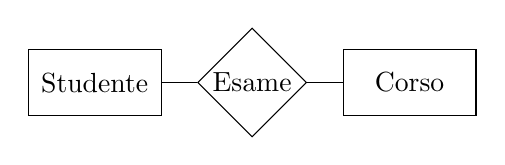
\begin{tikzpicture}[auto]

  \node[entity] (studente) at (0,0) {Studente};
  \node[entity] (corso) at (4,0) {Corso};
    \node[relationship] at (2,0) {Esame}
    edge (corso)
    edge (studente);
    \end{tikzpicture}
\end{center}

Si possono avere associazioni diverse tra stesse entità.

\begin{center}
    \begin{tikzpicture}[auto]

  \node[entity] (impiegato) at (0,0) {Impiegato};
  \node[entity] (città) at (4,0) {Città};
    
    \node[relationship] at (2,0) {Risiede}
    edge (corso)
    edge (studente);

    \node[relationship] at (2,-2) {Lavora}
    edge (corso)
    edge (studente);
    
    \end{tikzpicture}
\end{center}

Si possono avere associazioni ricorsive.

\begin{center}
    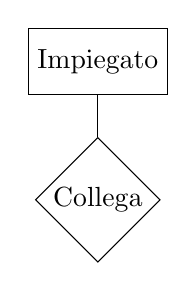
\begin{tikzpicture}[ node distance =5 em]

  \node[entity] (impiegato) at (0,0) {Impiegato};
    \node[relationship] (collega) [below of = impiegato] {Collega}
    edge (impiegato);
    \end{tikzpicture}
\end{center}

Le occorrenze di un'associazione sono le coppie o le triple  delle occorrenze delle entità. La semantica delle associazioni \textbf{\textit{non}} permette ripetizioni.

\subsection{Cardinalità delle associazioni}

La \textcolor{blue}{cardinalità} delle associazioni descrive il numero minimo e massimo di possibili occorrenze dell'associazione a cui le occorrenze delle entità partecipano.

\begin{center}
    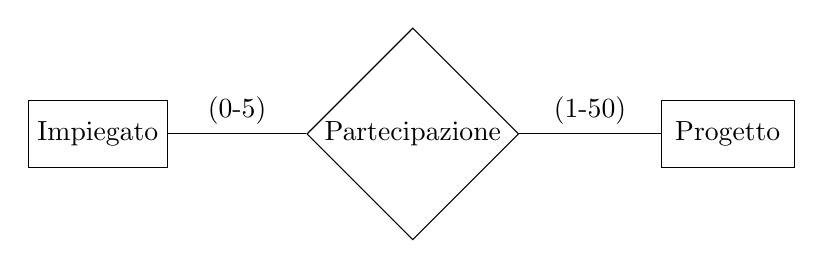
\begin{tikzpicture}[node distance = 6 em]

  \node[entity] (impiegato) at (0,0) {Impiegato};
  \node[entity] (progetto) at (8,0) {Progetto};
    
    \node[relationship] (partecipazione) at (4,0) {Partecipazione};
    \path (partecipazione) edge [above] node {(0-5)} (impiegato)
    edge [above] node {(1-50)}	(progetto);
    
    \end{tikzpicture}
\end{center}

\section{Attributi}

Gli \textcolor{blue}{attributi} descrivono proprietà di entità o associazioni. Ogni attributo è caratterizzato da un dominio che comprende i valori ammissibili. Si possono avere attributi con lo stesso nome, ma devono essere legati a entità/associazioni diverse. Gli attributi sono rappresentati da pallini vuoti.

\begin{center}
    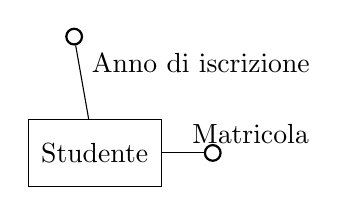
\begin{tikzpicture}[auto]

  \node[entity] (studente) at (0,0) {Studente};
    \tikzstyle{knode}=[circle,draw=black,thick,inner sep=2pt]
    \node (n1) at (0:1.5cm) [knode] {};
    \node (n2) at (100:1.5cm) [knode] {};

\path (n1) edge [above right] node {Matricola} (studente);
\path (n2) edge [above right] node {Anno di iscrizione} (studente);
    \end{tikzpicture}
\end{center}

\subsection{Cardinalità degli attributi}

Anche gli attributi possono avere una \textcolor{blue}{cardianlità}:

\begin{itemize}
    \item 0, l'attributo è opzionale;
    \item 1, l'attributo è obbligatorio;
    \item n, l'attributo è multivalore.
\end{itemize}

\begin{center}
    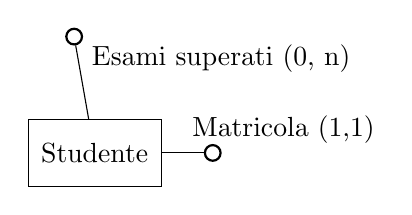
\begin{tikzpicture}[auto]

  \node[entity] (studente) at (0,0) {Studente};
    \tikzstyle{knode}=[circle,draw=black,thick,inner sep=2pt]
    \node (n1) at (0:1.5cm) [knode] {};
    \node (n2) at (100:1.5cm) [knode] {};

\path (n1) edge [above right] node {Matricola (1,1)} (studente);
\path (n2) edge [above right] node {Esami superati (0, n)} (studente);
    \end{tikzpicture}
\end{center}

\subsection{Attributi composti}

Gli \textcolor{blue}{attributi composti} raggruppano attributi simili. Per esempio indirizzo può raggruppare via e numero civico.
\chapter{Laboratorio 2}

\section{Identificatori delle entità}

Gli \textcolor{blue}{identificatori} delle entità servono per identificarle univocamente. Possono essere:
\begin{itemize}
    \item \textcolor{blue}{interni:} sono costituiti dagli attributi delle entità;
    \item \textcolor{blue}{esterni:} sono costituiti da attributi delle entità più entità esterne, tramite associazioni.
\end{itemize}

Gli identificatori sono rappresentati come pallini pieni.

\begin{center}
    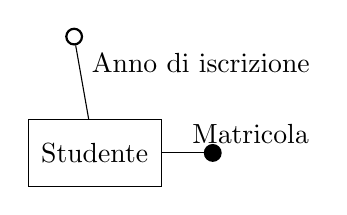
\begin{tikzpicture}[auto]

  \node[entity] (studente) at (0,0) {Studente};
    \tikzstyle{knode}=[circle,draw=black,thick,inner sep=2pt]
    \tikzstyle{knode_i}=[circle,draw=black, fill = black,thick,inner sep=2pt]
    \node (n1) at (0:1.5cm) [knode_i] {};
    \node (n2) at (100:1.5cm) [knode] {};

\path (n1) edge [above right] node {Matricola} (studente);
\path (n2) edge [above right] node {Anno di iscrizione} (studente);
    \end{tikzpicture}
\end{center}

Se sono necessari più attributi si rappresentano con una sbarra con pallino nero sopra gli attributi necessari.

Ogni entità deve avere almeno un identificatore e ogni attributo che fa parte di un identificatore deve avere  cardinalità (1, 1).

\section{Generalizzazione}

La \textcolor{blue}{generalizzazione} mette in relazione una o più entità $E_1$, $E_2$, ..., $E_n$ con una entità E che le comprende come casi particolari:

\begin{itemize}
    \item E è \textcolor{blue}{generalizzazione} di $E_1$, $E_2$, ..., $E_n$;
    \item $E_1$, $E_2$, ..., $E_n$ sono \textcolor{blue}{specializzazioni} di E;
\end{itemize}

Ogni occorrenza di $E_1$, $E_2$, ..., $E_n$ è anche occorrenza di E. Ogni proprietà di E è anche proprietà di $E_1$, $E_2$, ..., $E_n$.

Una generalizzazione può essere:
\begin{itemize}
    \item \textcolor{blue}{totale} se ogni occorrenza dell'entità genitore è occorrenza di almeno una delle entità figlie;
    \item \textcolor{blue}{parziale} se non è totale;
    \item \textcolor{blue}{esclusiva} se ogni occorrenza dell'entità genitore è occorrenza di al più una delle entità figlie;
    \item \textcolor{blue}{sovrapposta} se non è esclusiva.
\end{itemize}

\section{Documentazione schemi concettuali}

\begin{itemize}
    \item \textcolor{blue}{Descrizione di concetti:} dizionari per entità e associazioni;
    \item \textcolor{blue}{Vincoli non esprimibili in ER:} di integrità o di derivazione.
\end{itemize}
\chapter{Laboratorio 3}

\section{Progettazione concettuale}

L'analisi inizia con i primi requisiti raccolti (in linguaggio naturale).
Le possibili fonti sono:
\begin{itemize}
    \item utenti, attraverso documenti o interviste;
    \item documentazione già esistente, come normative o regolamenti interni;
    \item realizzazioni preesistenti.
\end{itemize}

\subsection{Acquisizione tramite interviste}
Utenti diversi possono fornire informazioni diverse (complementari o contradditorie). Gli utenti ad alto livello vedono il quadro generale, mentre gli utenti a basso livello vedono i dettagli.

\subsection{Suggerimenti per la progettazione}

Se un concetto ha proprietà significative e descrive oggetti con esistenza autonoma è un'entità.

Se un concetto è semplice e non ha proprietà è un attributo.

Se un concetto lega tra loro due o più concetti è un'associazione.

Se un concetto è un caso particolare di un altro concetto è una generalizzazione.

\subsection{Requisiti (documentazione descrittiva)}

Si deve scegliere il corretto livello di astrazione, standardizzare la struttura delle frasi ed evitare frasi contorte. Si devono unificare i termini eliminando omonimi\footnote{Hanno lo stesso nome, ma si riferiscono a concetti diversi} e sinonimi\footnote{Hanno nomi diversi, ma si riferiscono allo stesso concetto}, rendendo espliciti i riferimenti tra i termini. Si deve costruire un \textcolor{blue}{glossario dei termini} (tabella).

\section{Pattern di progettazione}

Sono soluzioni progettuali pronte per problemi comuni\footnote{Per la spiegazione in dettaglio si rimanda alle slide}:

\begin{itemize}
    \item Reificazione di attributo di entità: è la trasformazione di un attributo in un'identità;
    \item Part-of: due casi, il primo nel quale una parte non può esistere senza l'intero e il secondo in cui la parte può esistere senza l'intero;
    \item Instance-of: rappresenta il concetto istanza-classe;
    \item Reificazione di un'associazione binaria: si trasforma l'associazione binaria in un'entità;
    \item Reificazione di un'associazione ricorsiva: si trasforma l'associazione ricorsiva in un'entità;
    \item Reificazione di associazione ternaria: si trasforma l'associazione ternaria in un'entità;
    \item Reificazione di attributo di associazione;
    \item Caso particolare di un'entità: livelli diversi della generalizzazione partecipano ad associazioni diverse;
    \item Storicizzazione di un’entità: si usa la generalizzazione per rappresentare le informazioni correnti e contemporaneamente tenere traccia dello storico;
    \item Storicizzazione di un’associazione;
    \item Evoluzione di un concetto: si usa la generalizzazione per rappresentare l’evoluzione di un concetto mettendo nel genitore gli attributi e le associazioni comuni.
\end{itemize}

\section{Strategie di progetto}

\paragraph{Top-Down:} si individuano i concetti più importanti e si procede per raffinamenti successivi. Essa è conveniente perchè permette di trascurare momentaneamente alcuni dettagli, ma la si può utilizzare solo quando si ha una visione generale del progetto.

\paragraph{Bottom-Up:} le specifiche vengono divise in parti più semplici e poi unite alla fine. Questa strategia è adatta per i progetti di gruppo, ma l'integrazioni di varie parti può essere difficoltosa.

\paragraph{Inside-Out:} è una variante della Bottom-Up in cui si parte dai concetti più importanti e ci si espande a macchia d'olio. Non richiede integrazione, ma è necessario rivisitare periodicamente i requisiti per essere certi di rappresentare tutti i concetti.

\paragraph{Mista:} nella realtà si procede con una soluzione ibrida.

\section{Qualità di uno schema concettuale}

\paragraph{Correttezza:} devono essere utilizzati propriamente i costrutti messi a disposizione dal modello concettuale di riferimento.

\paragraph{Completezza:} deve modellare tutte le specifiche.

\paragraph{Leggibilità:} deve poter essere compreso in maniera immediata.

\paragraph{Minimalità:} le specifiche devono presentarsi una volta sola.
\chapter{Laboratorio 4}

\section{Progettazione logica}

La \textcolor{blue}{progettazione logica} è la fase successiva alla progettazione concettuale. 

Dati in ingresso: 
\begin{itemize}
    \item schema concettuale;
    \item informazioni sul carico applicativo;
    \item modello logico che si vuole adottare.
\end{itemize}

Dati in uscita: 
\begin{itemize}
    \item schema logico;
    \item vincoli di integrità;
    \item Documentazione associata.
\end{itemize}

Si può dividere in due sottofasi: la ristrutturazione dello schema concettuale (ER) e la traduzione verso il modello logico con relative ottimizzazioni.

\section{Ristrutturazione dello schema ER}

La \textcolor{blue}{ristrutturazione dello schema ER} serve a semplificare la traduzione nel modello logico e a ottimizzare le prestazioni. Si usano due indicatori per tenere traccia delle prestazioni: il tempo (numero di occorrenze visitate per un'operazione nel DB) e lo spazio (quantità di memoria per rappresentare i dati). Per poter valutare questi parametri si ha bisogno di alcune informazioni: il volume dei dati (numero di occorrenze e dimensione degli attributi) e le caratteristiche delle operazioni (se interattive o di batch, la frequenza e il numero di entità/associazioni coinvolte). Queste informazioni  vengono rappresentate su apposite tavole.

Per la ristrutturazione dello schema concettuale si possono seguire i seguenti passi.

\subsection{Analisi delle ridondanze}

Una \textcolor{blue}{ridondanza} è un'informazione significativa, ma ricavabile da altre informazioni. Si deve decidere se eliminare le ridondanze o mantenerle, con un calcolo. Le ridondanze rendono più efficienti le operazioni di interrogazione/lettura dei dati, ma rendono meno efficiente l'inserimento e la modifica dei dati, inoltre occupano spazio in memoria.

\subsection{Eliminazione delle generalizzazioni}

Le generalizzazioni non sono rappresentabili nel modello relazionale per cui vanno sostituite con entità, associazioni o regole aziendali (\textit{business rules}). In generale si hanno tre modi per eliminare una generalizzazione:

\begin{itemize}
    \item si accorpano i figli della generalizzazione nel genitore ("uccidendo" le entità figlie);
    \item si accorpa il genitore della generalizzazione nei figli ("uccidendo" l'entità genitore);
    \item si sostituisce la generalizzazione con associazioni, aggiungendo eventuali business rules.
\end{itemize}

Si possono anche adottare soluzioni ibride.

\subsection{Partizionamento di concetti}

Si separano attributi di uno stesso concetto ai quali si accede in operazioni diverse e si accorpando attributi di concetti diversi a cui si accede con le medesime operazioni. Spesso è possibile rimandare questo problema alla fase di progettazione fisica (che non è argomento di questo corso).

\subsection{Scelta degli identificatori principali}

Si devono scegliere gli identificatori che diventeranno chiave primaria seguendo alcuni criteri:

\begin{itemize}
    \item assenza di opzionalità;
    \item semplicità;
    \item utilizzo nelle operazioni più frequenti/importanti.
\end{itemize}

Se nessun identificatore rispetta questi criteri si devono introdurre nuovi attributi (per esempio codici) che serviranno da chiave primaria.

\subsection{Attributi composti e attributi multivalore}

Si possono trasformare gli attributi multivalore, reificando l’attributo e aggiungendo un’associazione. Gli attributi composti non sono rappresentabili direttamente in relazionale e devono essere trasformati.

\section{Traduzione verso il modello relazionale}

Le idee di base sono due:
\begin{itemize}
    \item le entità diventano relazioni con gli stessi attributi delle entità;
    \item Le associazioni diventano relazioni con attributi delle associazioni + gli identificatori delle entità coinvolte
\end{itemize}

Si devono dare nomi più espressivi agli attributi della chiave della relazione che rappresenta l’associazione. 

La traduzione non riesce a tener conto delle cardinalità minime delle associazioni molti a molti. La traduzione dell’associazione uno a molti riesce a rappresentare efficacemente la cardinalità minima della partecipazione che ha 1 come cardinalità massima (se è 0 ammette valori nulli, se è uno non ammette valori nulli). L’identificazione esterna è sempre su un’associazione uno a molti o un’associazione uno a uno.
\afterpage{\blankpage}
\chapter{Appendice - SQL}

In questo capitolo verranno messi tutti i concetti della parte di laboratorio su SQL. Tutte le nozioni di seguito sono applicabili a PostgreSQL, ma non tutte sono applicabili ad altri fornitori (es. Oracle).

\paragraph{SQL come linguaggio dichiarativo.}   In SQL l'utente deve definire \textit{cosa} vuole ottenere e il DBMS si occupa del \textit{come} ottenerlo. Una query SQL viene analizzata da un ottimizzatore del DBMS e trasformata per essere eseguita in modo efficiente (ragion per cui non ci si preoccuperà troppo dell'efficienza della scrittura delle query).

\section{Sintassi}

La struttura essenziale è la seguente:

\begin{lstlisting}[style=SQL, caption=Struttura base di una query]
SELECT ListaAttributi

[FROM ListaTabelle]

[WHERE Condizione];
\end{lstlisting}

Questo comando restituisce una tabella con gli attributi di \textit{ListaAttributi} del prodotto cartesiano delle tabelle in \textit{ListaTabelle} che rispettino la \textit{Condizione} (che è opzionale). Nella clausola select si possono scrivere espressioni riguardo qualsiasi attributo. Di seguito alcuni esempi di comandi con relative spiegazioni.

\paragraph{Esempio semplice:} Dà come risultato una tabella con tutti gli attributi di \textit{Tabella} utilizzando le sue tuple.

\begin{lstlisting}[style=SQL, caption=Semplice query]
SELECT *

FROM Tabella;
\end{lstlisting}

\paragraph{Esempio selezione:} Dà come risultato una tabella con tutti gli attributi dopo aver applicato una selezione\footnote{vedi \ref{Selezione}} in base all'attributo A3.

\begin{lstlisting}[style=SQL, caption=Semplice selezione]
SELECT *

FROM Tabella

WHERE A3 <= 20;
\end{lstlisting}

\paragraph{Esempio proiezione:} Dà come risultato una tabella con le stesse tuple di \textit{Tabella} a cui è stata apllicata una proiezione\footnote{vedi \ref{Proiezione}} su A1 e A2. 

\begin{lstlisting}[style=SQL, caption=Semplice proiezione]
SELECT A1, A2
    
FROM Tabella;
\end{lstlisting}

\section{Definizione di Dati}

Ci sono una serie di domini per definire i dati, inoltre è possibile definire dei propri domini (semplici, solamente a scopo di astrazione).

\paragraph{Stringhe.}

\begin{itemize}
    \item lunghezza fissa: char(length). Per esempio char(20) è una stringa lunga \textit{\textbf{esattamente}} 20 caratteri;
    \item lunghezza variabile: varchar (max\_length). varchar(20) è una stringa lunga \textit{\textbf{al massimo}} 20 caratteri.
\end{itemize}

\paragraph{Numeri esatti.}

\begin{itemize}
    \item numeri decimali: decimal(precisione, scala)/numeric(precisione, scala). La precisione è il numero totale di cifre decimali, la scala è il numero di cifre decimali dopo la virgola (sono entrambe opzionali);
    \item numeri interi: smallint (almeno 16 bit, con segno)/integer (almeno 32 bit, con segno)/bigint (almeno 64 bit, con segno).
\end{itemize}

\paragraph{Numeri approssimati.}

\begin{itemize}
    \item float(precisione). La precisione è il numero di cifre binarie per la mantissa (opzionale);
    \item real/double precision.
\end{itemize}

\paragraph{Istanti temporali.}

\begin{itemize}
    \item date: si usa \textit{date} che comprende year, month, day;
    \item orari: si usa \textit{time}(precisione) che comprende hour, minute, second;
    \item Per specificare data e orario si usa \textit{timestamp} (precisione) che comprende year, month, day, hour, minute, second.
\end{itemize}

\paragraph{Intervalli.}

\begin{itemize}
    \item durate in anni: interval year;
    \item durate in anni e mesi: interval year to month;
    \item durate in giorni, ore, minuti, secondi e centesimi di secondo: interval day to second (2),
    \item alcune durate in cui non è possibile passare in modo preciso non sono permesse (per esempio non si può passare da mesi a giorni perchè i mesi hanno durate diverse).
\end{itemize}

\paragraph{Ulteriori domini.}

\begin{itemize}
    \item vero/falso: boolean;
    \item immagini, video, file: blob;
    \item lunghi file di testo: clob.
\end{itemize}

\section{Definizione di tabelle}

La sintassi per la creazione di una tabella è la seguente;

\begin{lstlisting}[style=SQL, caption=Creazione tabella]
CREATE TABLE NomeTabella (
    
    NomeAttributo1 Dominio1 [ValoreDefault1][Vincoli1]

    NomeAttributo2 Dominio2 [ValoreDefault2][Vincoli2]

    ...

    NomeAttributoN DominioN [ValoreDefaultN][VincoliN]
    
);
\end{lstlisting}

Il ValoreDefault è un valore opzionale che verrà usato, se nel momento dell'inserimento, di una tupla non viene specificato alcun valore. Se non viene scelto un ValoreDefault si utilizza NULL.

Alcuni vincoli sono particolari:

\begin{itemize}
    \item \textbf{not null}: indica che il valore NULL non è ammesso (l'attributo è obbligatorio). Se l'attributo non viene specificato in fase di inserimento (e non è presente un ValoreDefault) l'operazione è annullata;
    \item \textbf{unique}: il valore di un attributo o di una superchiave deve essere unico. Eccezzione per il valore NULL. Sintassi su più attributi: unique (A1, A2,...,AN);
    \item \textbf{primary key}: un attributo o un insieme di attributi che fungono da chiave primaria. Questi attributi non possono essere NULL e può esserci solo un vincolo primary key per tabella;
    \item \textbf{Vincolo di integrità referenziale}: crea un vincolo tra i valori di uno (o più) attributi della tabella (interna) su cui è definito e uno (o più) attributi di un’altra tabella (esterna).
\end{itemize}

Sintassi del vincolo di integrità referenziale:

\begin{lstlisting}[style=SQL, caption=Integrità referenziale]
A1, Dominio1,
    
A2, Dominio2,
    
...

foreign key (A1, A2,...)

references NomeTabellaEsterna (B1, B2,...)
\end{lstlisting}

Ci sono casi in cui viene violata l'integrità (inserimento, modifica, cancellazione). Alcuni casi rifiutano l'operazione (se cambia la tabella interna), altri casi prevedono varie possibilità di reazione:

\begin{itemize}
    \item \textbf{cascade}: il nuovo valore dell’attributo della tabella esterna viene riportato in tutte le corrispondenti
righe della tabella interna (in caso di modifica) o tutte le righe della tabella interna corrispondenti alla riga cancellata nella tabella esterna vengono cancellate (in caso di cancellazione);
\item \textbf{set null}: all’attributo referente della tabella interna viene assegnato il valore NULL;
\item \textbf{set default}: all’attributo referente della tabella interna viene assegnato il valore di default;
\item \textbf{no action}: la modifica/cancellazione è rifiutata.
\end{itemize}
\pagebreak
\paragraph{Sintassi per la modifica (subito dopo il vincolo):} si usa update.

\begin{lstlisting}[style=SQL, caption=]
ON UPDATE Reazione
\end{lstlisting}

\paragraph{Sintassi per la cancellazione (subito dopo il vincolo):}  si usa delete

\begin{lstlisting}[style=SQL, caption=]
ON DELETE Reazione
\end{lstlisting}

Inoltre, si può dare il nome a un vincolo (per i dettagli sui vincoli vedere \ref{Vincoli}): 

\begin{lstlisting}[style=SQL, caption=]
CONSTRAIN NomeVincolo DefinizioneVincolo
\end{lstlisting}

In SQL è possibile modificare definizioni di tabelle, domini e vincoli introdotti precedentemente usando i comandi \textbf{alter} (modifica), \textbf{drop} (cancellazione), \textbf{add} (aggiunta).
Per inserire nuove righe in una tabella si usa il comando \textbf{insert}.

\begin{lstlisting}[style=SQL, caption=Inserire nuove righe in una tabella]
INSERT INTO Tabella(A1, ..., AN) values
        (ValoreAttributo1, ..., ValoreAttributoN);
\end{lstlisting}

Se un attributo non viene inserito, non ha specificato un ValoreDefault e non è \textit{nullable} l'operazione viene rifiutata. Se si specificano i valori per tutte le colonne, la lista di attributi può essere omessa.
Per cancellare (con condizione) delle righe si usa il comando \textbf{delete}.
\begin{lstlisting}[style=SQL, caption=Cancellare righe in una tabella]
DELETE FROM Tabella WHERE Condizione
\end{lstlisting}

\paragraph{La clausola where.} La clausola where è costituita da un'espressione boolean in logica proposizionale.

Per confrontare stringhe è possibile usare l'operatore \textbf{like}, avendo accesso a caratteri speciali:
\begin{itemize}
    \item \_ (trattino basso): un carattere qualsiasi;
    \item \% (percentuale): una sequenza di caratteri qualsiasi maggiore o uguale a zero;
\end{itemize}

Per esempio: \_\%@gmail.\_\_\% può essere usato per identificare un indirizzo mail con almeno un carattere precedente @ e con un dominio di almeno 2 caratteri.

\paragraph{Ordinamento dei risultati.} Per ordinare i risultati di una query si usa la clausola \textbf{order by}. Specificando più attributi, a parità di primo attributo, vengono ordinate con il secondo attributo e così via. Si possono aggiungere asc (crescente )e desc (decrescente). Esempio:

\begin{lstlisting}[style=SQL, caption=Ordinare i risultati in una query]
ORDER BY A1 [asc / desc], 
A2 [asc / desc], ...
\end{lstlisting}

Le righe con valore NULL sono messe tutte insieme (o all'inizio o alla fine).

\paragraph{Gestione dei valori nulli.} Un attributo NULL è diverso da 0, stringa vuota o \textit{blank}. Un confronto con il valore NULL dà sempre Unknow nella logica a tre valori\footnote{vedi \ref{Logica a tre valori}}. Per cui si utilizzano i predicati \textbf{is null} e \textbf{is not null}. In alcuni casi è meglio trttare i valori NULL com 0, per cui si usa la funzione \textbf{coalesce}. Esempio:

\begin{lstlisting}[style=SQL, caption=I valori nulli]
SELECT A1, COALESCE (A2, 0)
FROM A;
\end{lstlisting}

\paragraph{Commenti.} I commenti su una riga iniziano con -- (doppio trattino). Per i commenti su più righe si usa /* commento */.

\section{DML: tipi di Join} 

Per eseguire interrogazioni che riguardano più tabelle si deve usare il join\footnote{vedi \ref{Join i} e \ref{Join e}}. La congiunzione avviene sui valori in comune tra le tabelle. Con il join, in SQL si possono avere righe duplicate (al contrario dell'algebra relazionale che prevede l'unicità delle tuple). Per evitare ciò si deve ricorrere alla parola chiave \textbf{distinct} subito dopo \textbf{select}. 
Il join inizia eseguendo il prodotto cartesiano sulle tabelle nella clausola \textbf{from} e vengono eliminate quelle che non rispettano la clausola \textbf{where}.
Ci sono tre modi per usare un join in SQL di seguito elencati tramite esempi.

\subsubsection{Join e clausola from.}

\begin{lstlisting}[style=SQL, caption=]
SELECT A1, A2, B1, C1, C2

FROM A, B, C;
\end{lstlisting}

\subsubsection{Join e clausola where.}

\begin{lstlisting}[style=SQL, caption=]
SELECT A1, A2, B1, C1, C2

FROM A, B, C

WHERE (A1 = B1 OR A1 = C1) AND A2 <= C2; 
\end{lstlisting}

\subsubsection{Join come parola riservata.}

\begin{lstlisting}[style=SQL, caption=Join]
SELECT *

FROM A [INNER] JOIN B ON A1 = B2

WHERE A3 = 'IT'  AND A2 = 25; 
\end{lstlisting}

La parola inner è opzionale, inoltre è possibile mettere in join più tabelle. Si possono anche effettuare join esterni mettendo prima di join left, right o full. 

Si può effettuare il join di una tabella con sè stessa (self join), ricordandosi di specificare degli alias per gli attributi. Esempio:

\begin{lstlisting}[style=SQL, caption=Self-Join]
\begin{center}
SELECT ...

FROM A JOIN A_1 ON A.A1 = A_1.A1

A.A2 <= A_1.A2 ... 
\end{lstlisting}

\section{DML: funzioni aggregate}

In SQL è possibile valutare proprietà e condizioni su gruppi di righe. Le funzioni aggregate prendono in considerazione gruppi di righe e danno come risultato un unico valore per gruppo. Non è possibile usare funzioni aggregate (che
considerano gruppi di righe) direttamente nella clausola where (che viene valutata per ogni riga). Non è possibile combinare funzioni aggregate (che restituiscono un unico valore) con attributi non aggregati che possono assumere valori diversi nello stesso gruppo. Di solito si usano conteggio, somma, massimo e minimo.

\textbf{count(*)} conta il numero di righe (compresi valori NULL e valori duplicati). Si può specificare un nome per la colonna di questa interrogazione. Esempio:

\begin{lstlisting}[style=SQL, caption=Count]
SELECT COUNT(*) Nome

FROM A

WHERE A1 = 'UK';
\end{lstlisting}

\textbf{count(Attr)} conta il numero di valori non NULL per l'attributo Attr (si può usare il distinct per eliminare i duplicati). PostgreSQL non supporta count(distinct *).

\paragraph{Altre funzioni.}

\begin{itemize}
    \item sum(Attr): somma dei valori nella colonna Attr;
    \item avg(Attr): media dei valori nella colonna Attr;
    \item max(Attr): massimo dei valori nella colonna Attr;
    \item min(Attr): minimo dei valori nella colonna Attr.
\end{itemize}

\paragraph{Query con raggruppamento.} È possibile suddividere le righe di una tabella in più gruppi e applicare la funzione aggregata a ogni gruppo. È possibile considerare più di un attributo per formare raggruppamenti più specializzati. Per fare ciò si scrive al fondo \textbf{group by} e i nomi degli attributi, rispettando la seguente sintassi.

\begin{lstlisting}[style=SQL, caption=Query con raggruppamento]
SELECT SottinsiemeAttributiDiscriminanti,
    
FunzioneAggregata(AltroAttributo)

FROM Tabelle

WHERE Condizione

GROUP BY AttributiDiscriminanti;
\end{lstlisting}

\paragraph{Clausola having.} Nella clausola \textbf{having} vanno messe solo condizioni in cui compaiono funzioni aggregate (essa viene scritta dopo il \textbf{group by}. Esempio:

\begin{lstlisting}[style=SQL, caption=Having]
SELECT A1
    
FROM A

WHERE A2>=20

GROUP BY A1

HAVING COUNT(*) >= 2;
\end{lstlisting}

\section{DML: operatori insiemistici}

SQL mette a disposizione gli operatori insiemistici union, intersect, except corrispondenti agli operatori di unione, intersezione e differenza dell’algebra relazionale\footnote{vedi \ref{Op ins}}. Questi operatori rimuovono i duplicati. Se si vogliono mantenere si deve aggiungere la parola chiave \textbf{all}.

\subsubsection{Sintassi unione.}

\begin{lstlisting}[style=SQL, caption=Union]
SELECT EspressioneListaAttributi1
    
FROM ListaTabelle1

WHERE Condizioni1

UNION [ALL]

SELECT EspressioneListaAttributi2

FROM ListaTabelle2

WHERE Condizioni2;
\end{lstlisting}

\subsubsection{Sintassi intersezione.}

\begin{lstlisting}[style=SQL, caption=Intersect]
SELECT EspressioneListaAttributi1
    
FROM ListaTabelle1

WHERE Condizioni1

INTERSECT [ALL]

SELECT EspressioneListaAttributi2

FROM ListaTabelle2

WHERE Condizioni2;
\end{lstlisting}

\subsubsection{Sintassi differenza.}

\begin{lstlisting}[style=SQL, caption=Except]
SELECT EspressioneListaAttributi1
    
FROM ListaTabelle1

WHERE Condizioni1

EXCEPT [ALL]

SELECT EspressioneListaAttributi2

FROM ListaTabelle2

WHERE Condizioni2;
\end{lstlisting}

\section{DML: query nidificate}

In SQL si possono annidare sottoquery in query, ciò è utile per risolvere sottoproblemi. 
Esistono due tipologie di sottoquery:
\begin{itemize}
    \item semplici (o stratificate): è possibile valutare prima l’interrogazione più interna (una volta per tutte), poi, sulla base del suo risultato, valutare l’interrogazione più esterna;
    \item correlate (o incrociate): se l’interrogazione più interna fa riferimento a una delle tabelle appartenenti all’interrogazione più esterna. Per ciascuna riga candidata alla selezione nell’interrogazione più esterna, è necessario valutare nuovamente la sottoquery.
\end{itemize}

Se la sottointerrogazione restituisce più di un valore, per effettuare il confronto è necessario utilizzare uno dei quantificatori seguenti:
\begin{itemize}
    \item \textbf{any}: il predicato deve essere soddisfatto da almeno una riga restituita dalla sottointerrogazione;
    \item \textbf{all}: il predicato deve essere soddisfatto da tutte le righe restituite dalla sottointerrogazione, ma non viene quasi mai utilizzato perchè in presenza di valori NULL restituisce una query vuota.
\end{itemize}

\paragraph{IN e NOT IN.} Per verificare che un valore sia presente o meno in un insieme si usano le condizioni \textbf{in} e \textbf{not in}.

\paragraph{Sottointerrogazioni correlate.} SQL permette all’interrogazione annidata di fare riferimento al contesto relativo all’interrogazione più esterna (\textit{passaggio di binding}), permettendo di valutare un'espressione di una riga esaminata dalla query più esterna. Bisogna che gli attributi in query distinte siano visibili (dichiarati in select). In queste sottointerrogazioni si possono usare i costrutti \textbf{exist} (la riga in esame nella query più esterna soddisfa il predicato exists se la query annidata non restituisce l’insieme vuoto) e \textbf{not exist} (la riga in esame nella query più esterna soddisfa il predicato not exists se la query annidata restituisce l’insieme vuoto).

\end{document}